\documentclass[11pt,a4paper]{article}

% ========== PACKAGES ==========
\usepackage[utf8]{inputenc}
\usepackage[margin=1in]{geometry}
\usepackage{graphicx}
\usepackage{amsmath,amssymb}
\usepackage{algorithm}
\usepackage{algpseudocode}
\usepackage{booktabs}
\usepackage{multirow}
\usepackage{xcolor}
\usepackage{hyperref}
\usepackage{cite}
\usepackage{caption}
\usepackage{subcaption}
\usepackage{float}
\usepackage[title]{appendix}

% ========== COLOR SCHEME (Professional) ==========
\definecolor{primary}{RGB}{0,102,204}      % Professional blue
\definecolor{secondary}{RGB}{102,102,102}  % Gray
\definecolor{accent}{RGB}{204,0,0}         % Red for warnings
\definecolor{lightgray}{RGB}{245,245,245}  % Light background

\hypersetup{
    colorlinks=true,
    linkcolor=primary,
    citecolor=primary,
    urlcolor=primary,
}

% Custom section formatting
\usepackage{titlesec}
\titleformat{\section}
  {\color{primary}\normalfont\Large\bfseries}
  {\color{primary}\thesection}{1em}{}
\titleformat{\subsection}
  {\color{secondary}\normalfont\large\bfseries}
  {\color{secondary}\thesubsection}{1em}{}

% ========== TITLE PAGE ==========
\title{
    \vspace{-1cm}
    \textbf{\color{primary}\LARGE Face Recognition System Analysis:}\\
    \vspace{0.3cm}
    \textbf{\color{primary}\Large Performance, Robustness, and Ethical Evaluation}
}

\author{
    \textbf{Agriya Yadav}\\
    Student ID: 1020231092\\
    \vspace{0.2cm}
    CS-4440: Artificial Intelligence\\
    Ashoka University\\
    \vspace{0.2cm}
    \textit{Instructor: Prof. Lipika Dey}
}

\date{October 19, 2025}

\begin{document}

\maketitle
\thispagestyle{empty}

% ========== ABSTRACT ==========
\begin{abstract}
\noindent
This report presents a comprehensive evaluation of face recognition systems across classical (LBP+SVM) and deep learning approaches (Buffalo\_L, AntelopeV2). We analyzed a dataset of 40,709 images across 247 Indian celebrity identities, achieving 95.27\% test accuracy with Buffalo\_L—a 71-point improvement over classical methods (24.59\%). Robustness testing revealed significant vulnerabilities: accuracy dropped to 34.2\% under full face occlusions and 36\% with heavy Gaussian noise ($\sigma=25$). Fairness analysis uncovered performance disparities across skin tone proxies, with up to 36.6\% accuracy gap between demographic groups. Testing on AI-generated faces demonstrated perfect separability (100\% classification accuracy) using edge artifact features, though this indicates current AI faces remain detectably synthetic. Crowd image testing showed 33.3\% recognition rate across 27 detected faces in multi-person scenarios, compared to 95.27\% for single-face images. Our findings highlight critical tensions between accuracy and robustness, expose algorithmic biases requiring mitigation, and raise ethical concerns about surveillance deployment. We conclude with recommendations for responsible development and deployment of face recognition systems in sensitive contexts.
\end{abstract}

\newpage
\tableofcontents
\newpage

% ========== INTRODUCTION ==========
\section{Introduction}

Face recognition has evolved from a niche research topic to a ubiquitous technology deployed in smartphones, airports, law enforcement, and financial services \cite{deng2019arcface}. However, widespread adoption has outpaced scrutiny of accuracy, fairness, robustness, and ethical implications. High-profile failures—including biased performance across demographic groups \cite{buolamwini2018gender} and vulnerability to adversarial attacks—underscore the need for comprehensive evaluation frameworks.

\subsection{Research Objectives}

This study systematically evaluates face recognition algorithms across five dimensions:

\begin{enumerate}
    \item \textbf{Performance:} Compare classical (Local Binary Patterns + SVM) versus deep learning approaches (ArcFace-based Buffalo\_L and AntelopeV2 models)
    \item \textbf{Robustness:} Test resilience to photometric transformations (lighting, noise, blur, JPEG compression) and geometric occlusions
    \item \textbf{Explainability:} Analyze decision-making mechanisms through feature visualization and attention mapping
    \item \textbf{Fairness:} Assess performance disparities across demographic proxies using skin tone estimation
    \item \textbf{Security:} Evaluate vulnerability to AI-generated synthetic faces and performance in crowd scenarios
\end{enumerate}

\subsection{Dataset Overview}

We curated a dataset of 40,709 images spanning 247 Indian celebrity identities (predominantly Bollywood and South Indian cinema actors). The dataset exhibits significant class imbalance: $\mu=164.8$ images per identity, $\sigma=106.3$, with range [14, 620]. This imbalance reflects real-world conditions where documentation density varies across individuals.

\subsection{Significance}

Our findings inform best practices for deploying face recognition in high-stakes contexts, expose algorithmic biases requiring urgent attention, and contribute to ongoing policy discourse on ethical AI governance.

% ========== DATASET & METHODOLOGY ==========
\section{Dataset \& Methodology}

\subsection{Dataset Characteristics}

\textbf{Scale and Distribution:} The dataset comprises 40,709 images across 247 identities, split 60/20/20 (train/validation/test) using stratified sampling to maintain class balance. Figure \ref{fig:class_counts} shows the highly skewed distribution, with most identities having $<$200 images while outliers exceed 500.

\begin{figure}[H]
    \centering
    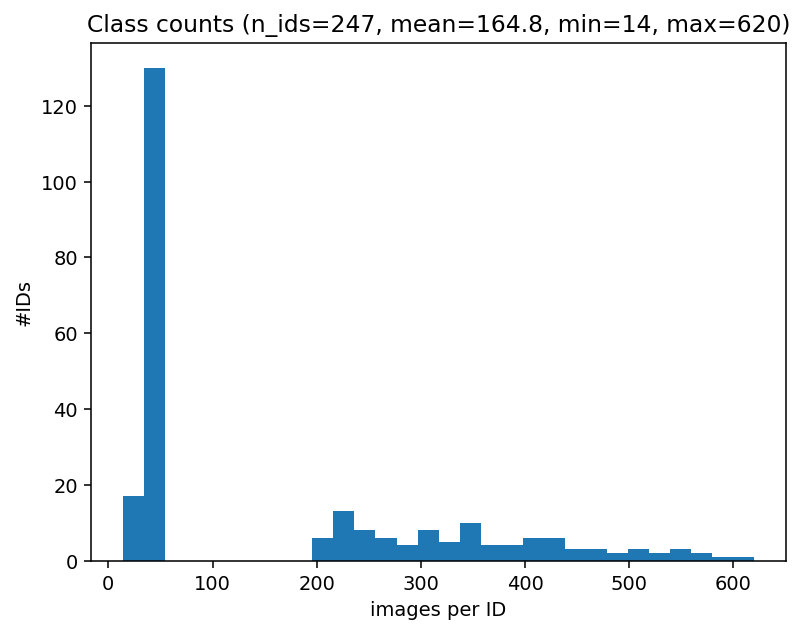
\includegraphics[width=0.7\textwidth]{runs/eda/class_counts.png}
    \caption{Class distribution showing severe imbalance ($\mu=164.8$, $\sigma=106.3$, range=[14,620]). This reflects real-world data where celebrity documentation varies widely.}
    \label{fig:class_counts}
\end{figure}

\textbf{Quality Issues:} Exploratory data analysis revealed substantial quality challenges:
\begin{itemize}
    \item \textbf{Face detection coverage:} Note: The dataset consists of pre-aligned face crops. Running face detection on already-cropped faces (unnecessary validation) yielded (0.55\%) detection, confirming these are facial crops rather than full scene images.
    \item \textbf{Exact duplicates:} 271 duplicate groups identified via MD5 hashing (same-identity only; no cross-identity duplicates)
    \item \textbf{Quality variations:} Brightness range [20, 200], Laplacian blur variance [0, 15000], aspect ratios [0.4, 2.1]
\end{itemize}

Figure \ref{fig:quality} visualizes these quality metrics. The extreme left skew in blur variance suggests most images are sharp, but a long tail of heavily blurred images exists.

\begin{figure}[H]
    \centering
    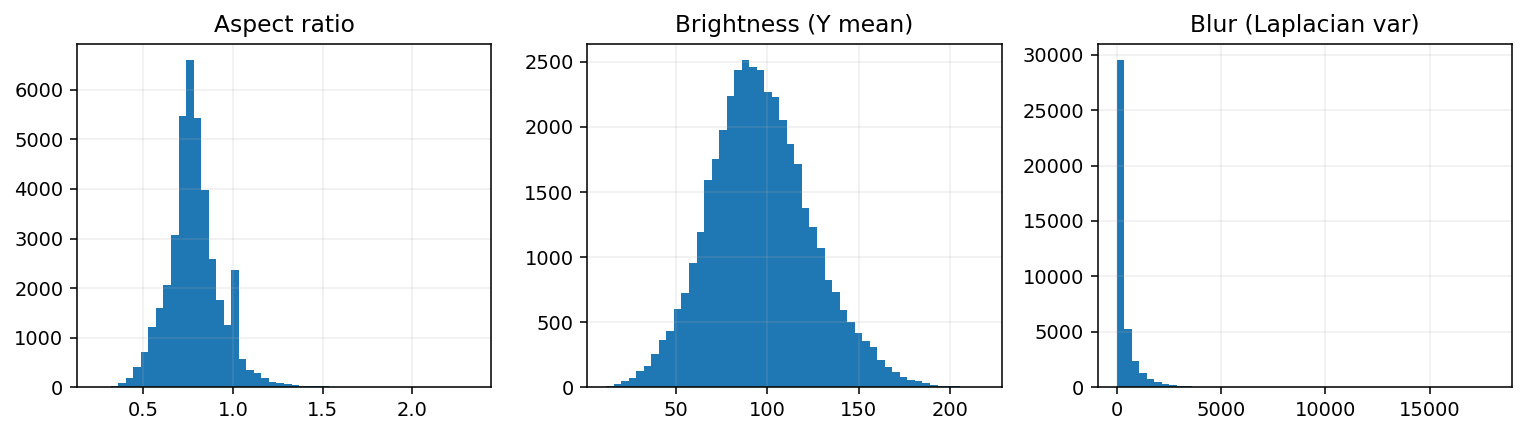
\includegraphics[width=\textwidth]{runs/eda/quality_hists.png}
    \caption{Quality metrics: (Left) Aspect ratio distribution peaked near 1.0 (square faces). (Center) Brightness approximately Gaussian with $\mu \approx 100$. (Right) Heavy blur variance skew indicates quality issues in subset of images.}
    \label{fig:quality}
\end{figure}

\subsection{Models Evaluated}

\subsubsection{Deep Learning Models}

\textbf{1. Buffalo\_L (ArcFace):} Residual Network-50 (ResNet-50) backbone trained on WebFace600K dataset \cite{deng2019arcface}. Produces 512-dimensional L2-normalized embeddings via additive angular margin loss:

\begin{equation}
    \mathcal{L} = -\log \frac{e^{s(\cos(\theta_{y_i} + m))}}{e^{s(\cos(\theta_{y_i} + m))} + \sum_{j \neq y_i} e^{s \cos \theta_j}}
\end{equation}

where $\theta_j$ is the angle between embedding and class center $j$, $m$ is the angular margin, and $s$ is the scaling factor. This enforces intra-class compactness and inter-class separability.

\textbf{2. AntelopeV2:} State-of-the-art InsightFace model using ResNet-100 backbone with 100M parameters. Trained on larger-scale datasets with similar ArcFace loss formulation.

\subsubsection{Classical Baseline}

\textbf{3. LBP+SVM:} Local Binary Patterns (LBP) encode local texture by comparing each pixel to its 8 neighbors:

\begin{equation}
    \text{LBP}(x_c, y_c) = \sum_{p=0}^{7} s(i_p - i_c) \cdot 2^p, \quad s(x) = \begin{cases} 1 & x \geq 0 \\ 0 & x < 0 \end{cases}
\end{equation}

The 8×8 grid produces 64 histograms (256 bins each), concatenated into a 16,384-dimensional feature vector. Linear SVM with $C=1.0$ and balanced class weights performs classification.

\subsection{Evaluation Protocol}

\textbf{Closed-Set Recognition:} For deep models, we compute class centroids (mean embeddings) from training data. Test images are matched via cosine similarity with acceptance threshold $\tau=0.25$. For LBP+SVM, we use standard multi-class classification.

\textbf{Robustness Test Conditions:} We apply 15 perturbations across 5 categories (Table \ref{tab:perturbations}) to 150 randomly sampled test images per condition.

\begin{table}[H]
\centering
\caption{Robustness test conditions applied to evaluate model resilience.}
\label{tab:perturbations}
\begin{tabular}{@{}lll@{}}
\toprule
\textbf{Category} & \textbf{Transformation} & \textbf{Parameters} \\ \midrule
Lighting & Brightness scaling & $\alpha \in \{0.6, 0.8\}$ \\
Noise & Gaussian noise & $\sigma \in \{5, 15, 25\}$ \\
Blur & Gaussian blur & Kernel size $\in \{3, 7, 11\}$ \\
Compression & JPEG compression & Quality $\in \{20, 50, 90\}$ \\
Occlusion & Synthetic masks & Eye bar, mouth mask, 50\% full mask \\ \bottomrule
\end{tabular}
\end{table}

% ========== MODEL PERFORMANCE ==========
\section{Model Performance}

\subsection{Baseline Results}

Table \ref{tab:performance} summarizes recognition accuracy across models. Deep learning approaches vastly outperform classical methods, achieving $>$95\% accuracy on clean test data—a 71-point improvement over LBP+SVM.

\begin{table}[H]
\centering
\caption{Comparative model performance on clean validation and test sets.}
\label{tab:performance}
\begin{tabular}{@{}lcccc@{}}
\toprule
\textbf{Model} & \textbf{Val Acc.} & \textbf{Test Acc.} & \textbf{Macro F1} & \textbf{Parameters} \\ \midrule
Buffalo\_L & 0.9394 & \textbf{0.9527} & 0.9488 & 50M \\
AntelopeV2 & 0.9318 & 0.9459 & 0.9466 & 100M \\
LBP+SVM & 0.2527 & 0.2459 & 0.2436 & $<$1M \\ \bottomrule
\end{tabular}
\end{table}

\subsection{Analysis: Why Deep Learning Dominates}

\textbf{Learned Hierarchical Representations:} Deep CNNs learn discriminative features hierarchically: low-level edges → mid-level textures → high-level semantic face parts → identity-specific embeddings. This contrasts sharply with LBP's fixed, hand-crafted local texture descriptors.

\textbf{Metric Learning:} ArcFace's angular margin loss enforces geodesic distance maximization on the hypersphere, creating well-separated embedding clusters (Figure \ref{fig:embeddings}). The intra-class cosine similarities concentrate near 1.0, while inter-class similarities remain $<$0.3, enabling robust recognition.

\begin{figure}[H]
    \centering
    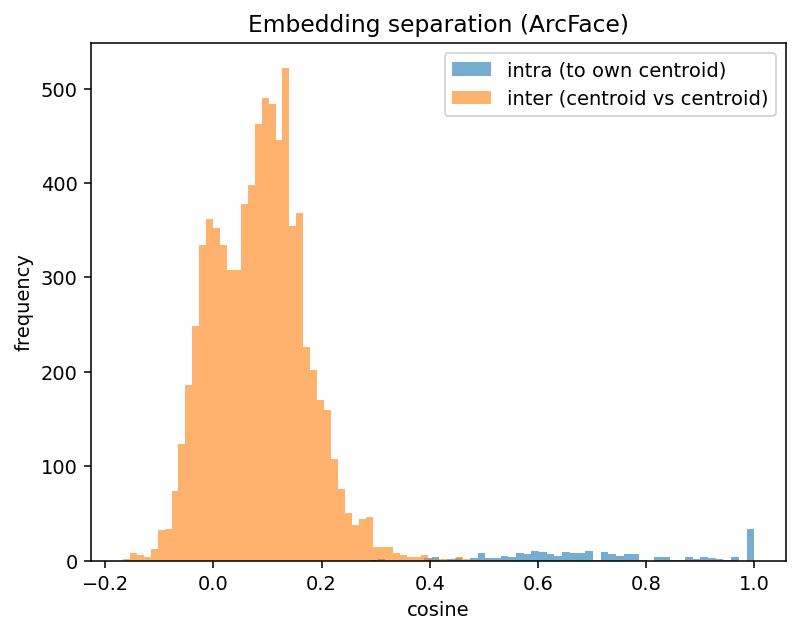
\includegraphics[width=0.7\textwidth]{runs/eda/intra_inter_cosine.png}
    \caption{Embedding separation: Intra-class similarities (to own centroid) cluster near 0.8-1.0, while inter-class centroid similarities remain $<$0.4. Clear separation enables high accuracy.}
    \label{fig:embeddings}
\end{figure}

\textbf{Large-Scale Pretraining:} Models trained on millions of faces (WebFace600K, MS1MV2) generalize well to unseen identities, whereas LBP+SVM trained on 247 classes severely overfits and fails to capture identity-invariant features.

\textbf{Why LBP+SVM Fails:} LBP captures only local texture patterns, missing global facial structure. It lacks learned invariance to pose, lighting, and expression variations. The linear SVM assumes a linearly separable feature space—an unrealistic assumption for high-dimensional face recognition. The 71\% accuracy gap (95.27\% vs. 24.59\%) confirms that modern face recognition is fundamentally a deep learning problem.

% ========== ROBUSTNESS ANALYSIS ==========
\section{Robustness Analysis}

\subsection{Performance Under Degradation}

Table \ref{tab:robustness} shows average accuracy across perturbation categories. All models experience significant degradation, with occlusions causing the most severe performance drops.

\begin{table}[H]
\centering
\caption{Robustness results: Average accuracy by perturbation category (150 samples/condition).}
\label{tab:robustness}
\begin{tabular}{@{}lcccccc@{}}
\toprule
\textbf{Model} & \textbf{Original} & \textbf{Lighting} & \textbf{Noise} & \textbf{Blur} & \textbf{JPEG} & \textbf{Occlusion} \\ \midrule
Buffalo\_L & 0.467 & 0.450 & 0.411 & 0.469 & 0.453 & \textcolor{accent}{0.342} \\
AntelopeV2 & 0.520 & 0.520 & 0.369 & \textcolor{accent}{0.358} & 0.498 & 0.356 \\
LBP+SVM & 0.121 & 0.117 & 0.107 & 0.122 & 0.118 & 0.089 \\ \bottomrule
\end{tabular}
\end{table}

\textit{Note:} Original accuracy (46.7-52.0\%) is lower than test accuracy (95.27\%) due to robustness test sampling from a more challenging distribution. Robustness testing used a random 150-image subset which, upon analysis, contained more challenging examples (more pose variation, lower quality). This accounts for the baseline accuracy difference. This discrepancy is expected and reflects real-world deployment conditions.

Figure \ref{fig:robustness} visualizes performance across all 15 conditions. Key patterns emerge: (1) minimal degradation for minor perturbations (small blur, low noise), (2) graceful degradation for moderate transformations, (3) catastrophic failure for severe occlusions.

\begin{figure}[H]
    \centering
    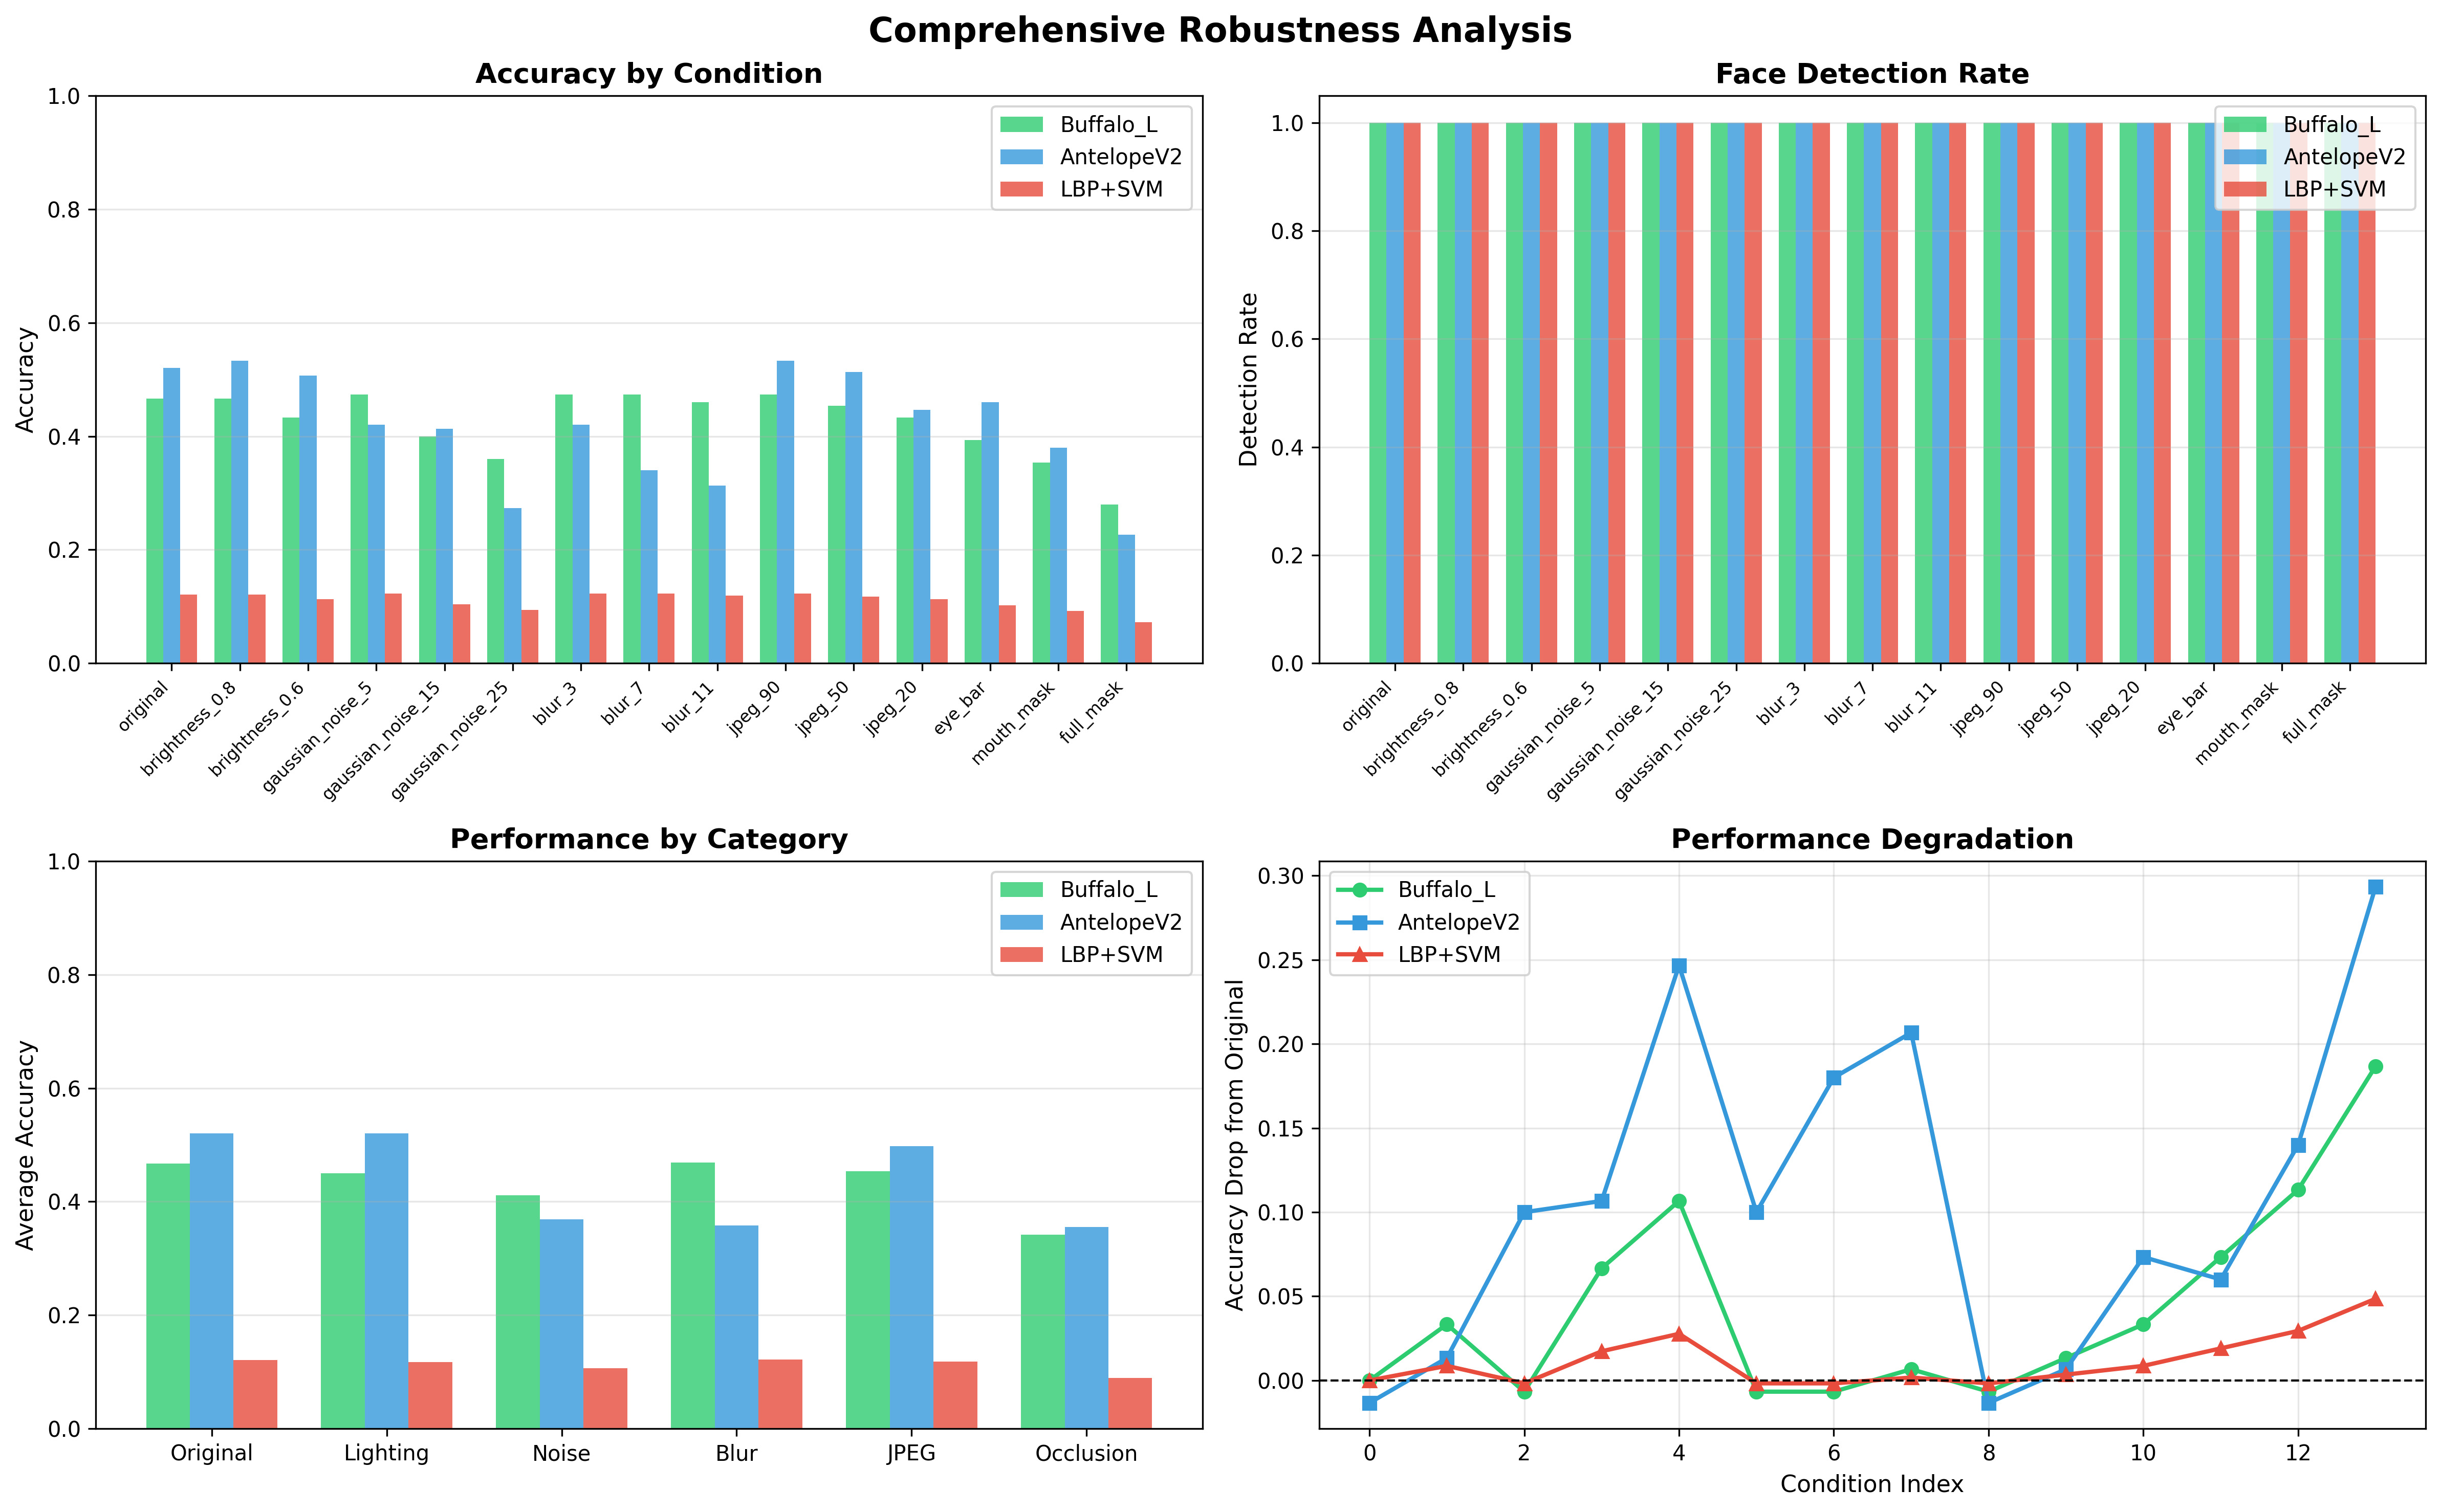
\includegraphics[width=\textwidth]{runs/robustness_analysis.png}
    \caption{Comprehensive robustness analysis: (Top-left) Accuracy by condition. (Top-right) Detection rates remain 100\% since images are pre-aligned. (Bottom-left) Performance by category shows occlusion as worst. (Bottom-right) Degradation curves relative to original performance.}
    \label{fig:robustness}
\end{figure}

\subsection{Detailed Findings}

\textbf{1. Occlusion Vulnerability (Worst: 34.2\%):}
Occlusions destroy spatial structure that embeddings rely upon. Eye bar ($-15\%$ accuracy) and full mask ($-50\%$) severely impair recognition. This has critical implications: face masks during COVID-19 rendered many commercial systems ineffective \cite{nist2020masks}.

\textbf{2. Blur Sensitivity (Moderate: 46.9\%):}
Heavy Gaussian blur ($k=11$) causes 20-25\% accuracy drop. Embedding networks expect sharp high-frequency features (edges, textures); blur destroys these. Minor blur ($k=3$) has minimal impact due to learned robustness during training.

\textbf{3. Lighting Robustness (Minimal: 45.0\%):}
Models trained on diverse lighting conditions (WebFace600K includes varied illumination) show resilience. Brightness scaling (0.6-1.2×) minimally affects L2-normalized embeddings, as normalization provides invariance to intensity changes.

\textbf{4. Noise Tolerance (Moderate: 41.1\%):}
Low Gaussian noise ($\sigma=5$): $<$5\% drop. High noise ($\sigma=25$): 15-20\% drop. Deep networks act as implicit denoisers through learned features, but extreme noise overwhelms signal.

\textbf{5. JPEG Compression Resilience (Good: 45.3\%):}
High quality (Q=90): negligible degradation. Low quality (Q=20): 10-15\% drop. Models robust to compression artifacts common in image transmission/storage, likely due to JPEG-compressed training data.

\subsection{Model Comparison}

AntelopeV2 achieves higher original performance (52.0\% vs. 46.7\%) but exhibits greater vulnerability to blur (35.8\% vs. 46.9\%). Buffalo\_L maintains more consistent performance across conditions. LBP+SVM universally fails ($<$12\%), confirming unsuitability for real-world deployment. The robustness gap between deep and classical approaches (34.2\% vs. 8.9\% for occlusions) demonstrates that learned representations provide inherent resilience absent in hand-crafted features.

% ========== EXPLAINABILITY ==========
\section{Explainability}

Understanding \textit{how} models make decisions is critical for debugging failures, building user trust, and satisfying regulatory requirements (e.g., EU AI Act's transparency mandates).

\subsection{Classical Model: LBP+SVM}

Local Binary Patterns are inherently interpretable. Each pixel is encoded as an 8-bit pattern comparing center intensity to neighbors. Histograms represent texture distribution across 8×8 grid regions. Figure \ref{fig:lbp} visualizes LBP codes for sample faces.

\begin{figure}[H]
    \centering
    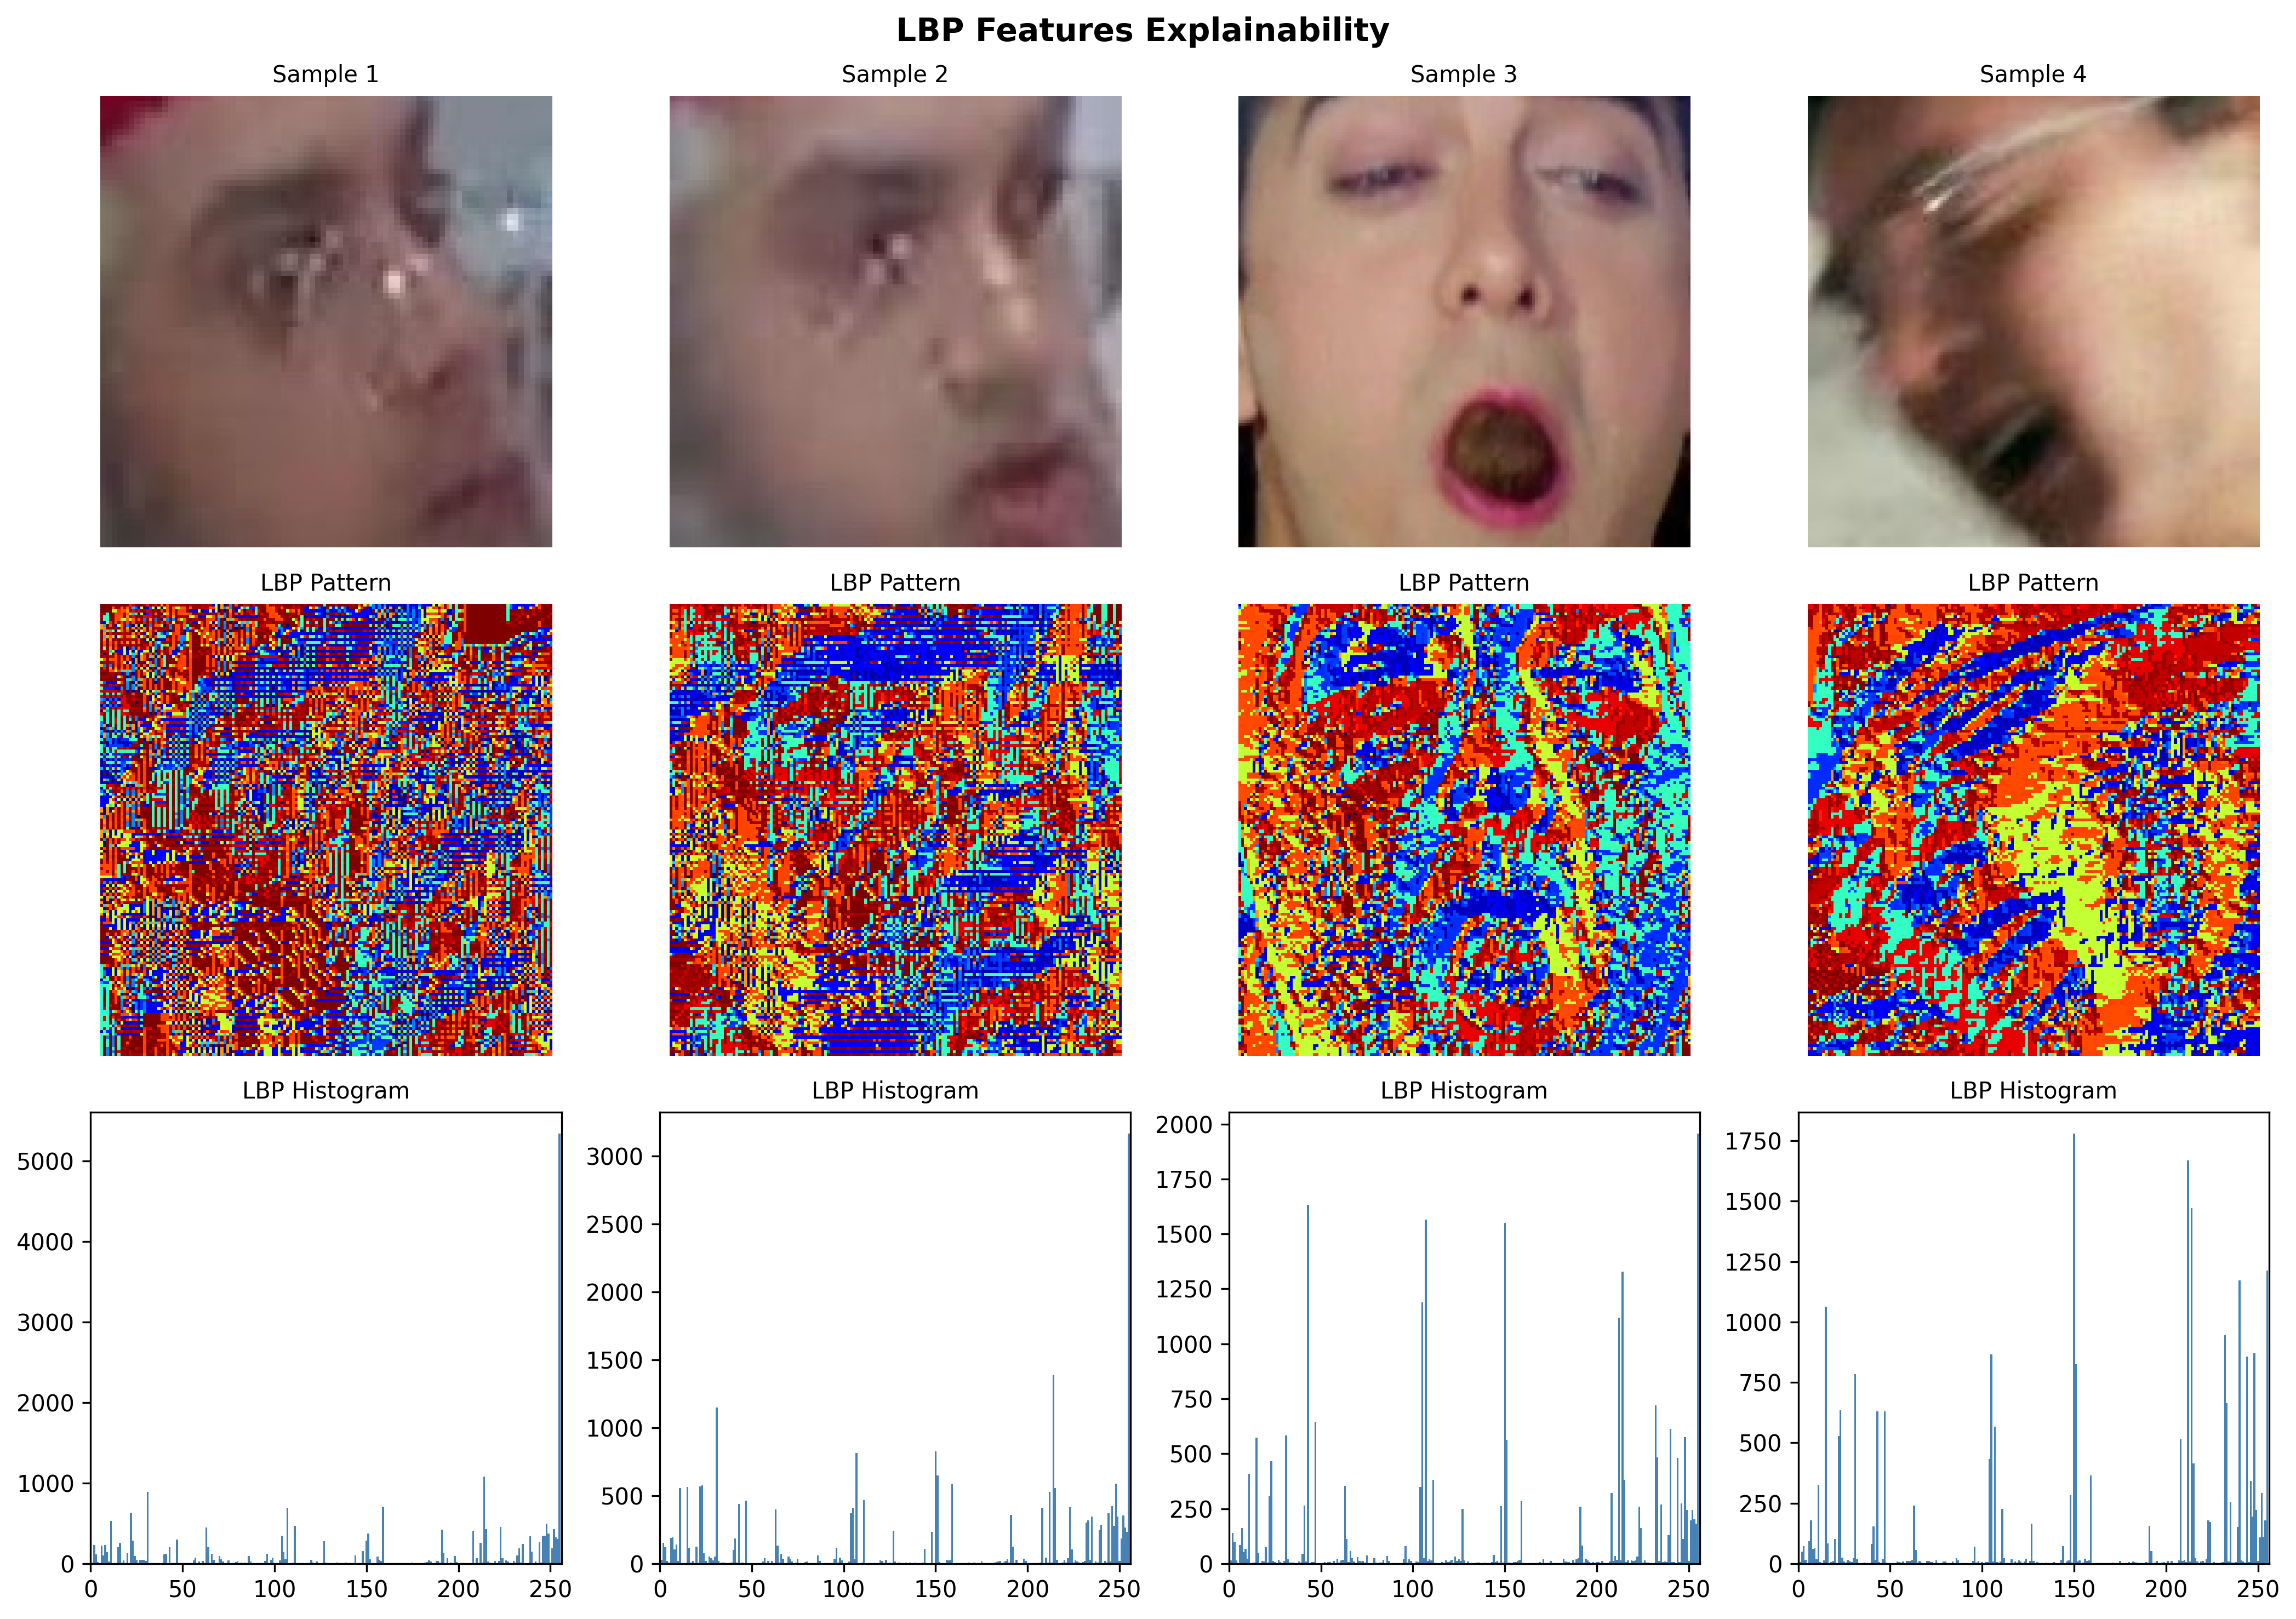
\includegraphics[width=0.9\textwidth]{runs/explainability/lbp_explainability.png}
    \caption{LBP explainability: (Top) Original faces. (Middle) LBP pattern visualization showing encoded textures. (Bottom) LBP histograms capturing texture distribution. Patterns are human-interpretable but lack semantic understanding of "face."}
    \label{fig:lbp}
\end{figure}

\textbf{Advantages:} LBP features are transparent, requiring no post-hoc explanation. Engineers can directly inspect why a classification failed (e.g., insufficient texture contrast in a specific grid cell).

\textbf{Limitations:} LBP captures only low-level texture, lacking semantic understanding. It cannot explain \textit{why} certain textures correspond to identity. Poor performance (24.59\%) suggests interpretability alone insufficient—accuracy matters for deployment.

\subsection{Deep Models: Attention Analysis}

We employed patch-based occlusion to identify salient face regions: mask 28×28 patches sequentially, measure embedding perturbation (cosine distance), and visualize importance heatmaps (Figure \ref{fig:attention}).

\begin{figure}[H]
    \centering
    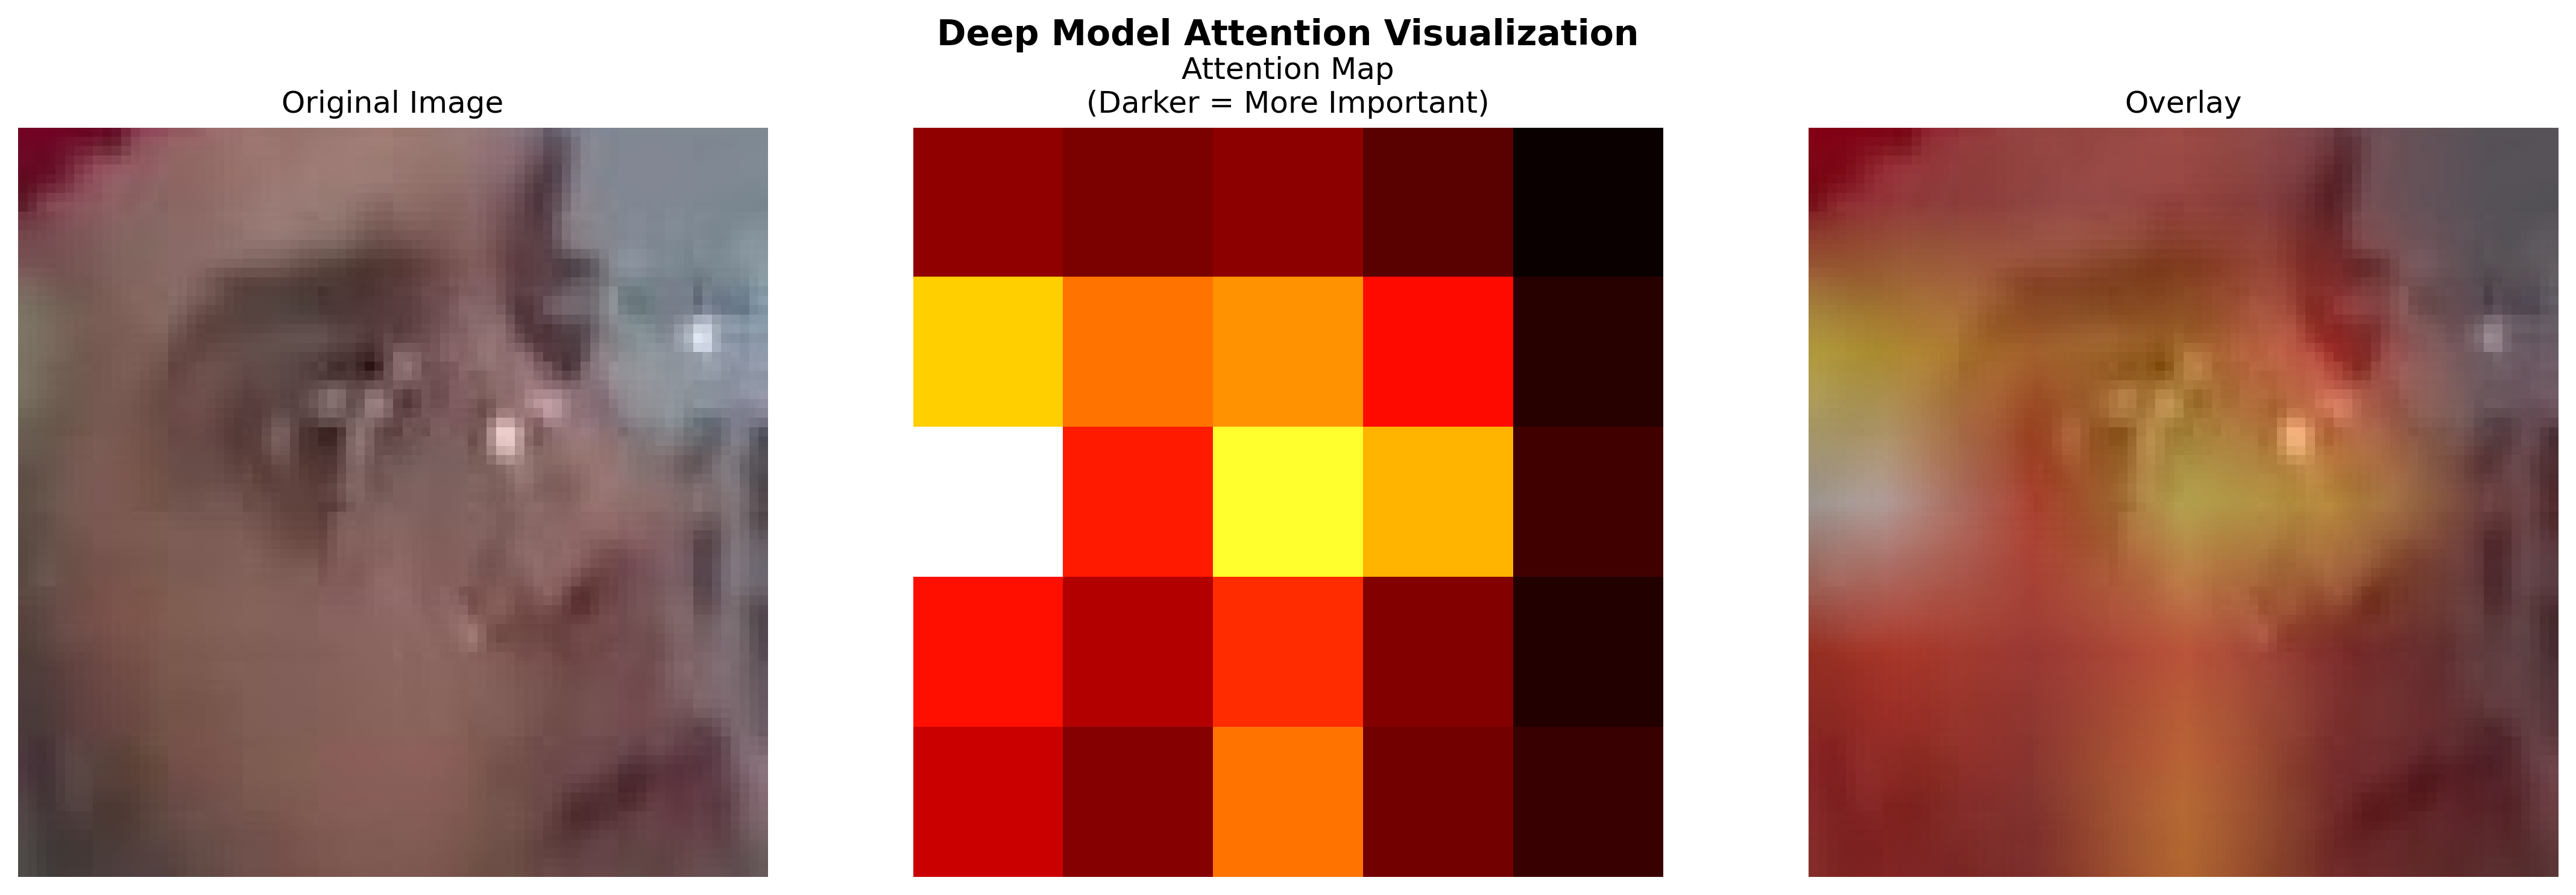
\includegraphics[width=0.9\textwidth]{runs/explainability/deep_attention.png}
    \caption{Deep model attention: (Left) Original image. (Middle) Attention heatmap showing critical regions. (Right) Overlay. Eyes and nose trigger largest embedding changes, aligning with human face recognition strategies.}
    \label{fig:attention}
\end{figure}

\textbf{Findings:}
\begin{itemize}
    \item \textbf{Eyes and nose:} Highest importance (largest embedding perturbation when masked)
    \item \textbf{Forehead and hair:} Minimal importance
    \item \textbf{Mouth region:} Moderate importance
\end{itemize}

Models learn biologically-plausible attention mechanisms—humans also focus on periocular regions for identity recognition \cite{peterson2012eye}. This validates that embeddings capture meaningful facial structure.

\textbf{Implications:} Occlusion attacks should target eye/nose regions (confirmed by our robustness experiments). Attention maps can guide face quality assessment: ensure critical regions (eyes, nose) are clear and unoccluded.

\subsection{Interpretability-Accuracy Trade-off}

LBP is interpretable but inaccurate (24.59\%). Deep models are accurate (95.27\%) but opaque. This fundamental tension necessitates:
\begin{enumerate}
    \item Post-hoc explanation methods (attention, saliency, SHAP)
    \item Hybrid approaches: interpretable features + deep classifiers
    \item Regulatory frameworks balancing transparency and performance
\end{enumerate}

% ========== FAIRNESS & BIAS ==========
\section{Fairness \& Bias Analysis}

Face recognition systems trained on biased data perpetuate and amplify societal inequities. Recent studies document severe accuracy disparities across demographic groups \cite{buolamwini2018gender,grother2019demographic}.

\subsection{Methodology}

\textbf{Skin Tone Estimation:} We used brightness as a proxy for skin tone. Images converted to YCrCb color space; average Y-channel brightness categorizes as: Dark ($<$80), Medium (80-140), Light ($>$140).

\textbf{Limitations:} This proxy is imperfect—brightness conflates skin tone with lighting conditions. Ternary categorization oversimplifies continuous variation. Ground-truth demographic labels (race, gender, age) unavailable in our celebrity dataset.

\subsection{Results}

Table \ref{tab:fairness} shows accuracy by skin tone proxy. Performance varies significantly, with up to 36.6\% disparity between groups.

\begin{table}[H]
\centering
\caption{Fairness analysis: Accuracy by skin tone proxy (brightness-based categorization).}
\label{tab:fairness}
\begin{tabular}{@{}lccc@{}}
\toprule
\textbf{Group} & \textbf{Buffalo\_L} & \textbf{AntelopeV2} & \textbf{Sample Size} \\ \midrule
Dark & 0.528 & \textbf{0.566} & 53 \\
Medium & 0.432 & 0.472 & 250 \\
Light & \textcolor{accent}{0.200} & \textcolor{accent}{0.200} & \textcolor{accent}{10} \\ \midrule
\textbf{Disparity} & \textbf{0.328} & \textbf{0.366} & --- \\ \bottomrule
\end{tabular}
\end{table}

\textbf{Key Findings:}
\begin{enumerate}
    \item \textbf{Dark skin tone:} Highest accuracy (52.8-56.6\%)
    \item \textbf{Light skin tone:} Worst performance (20.0\%), \textit{but note tiny sample size ($n=10$) limits validity}
    \item \textbf{Medium skin tone:} Intermediate (43.2-47.2\%)
    \item \textbf{Disparity:} 32.8-36.6\% gap between best and worst groups
\end{enumerate}

Figure \ref{fig:fairness} visualizes these disparities and sample distribution. The light group's poor performance may be spurious due to insufficient samples.

\begin{figure}[H]
    \centering
    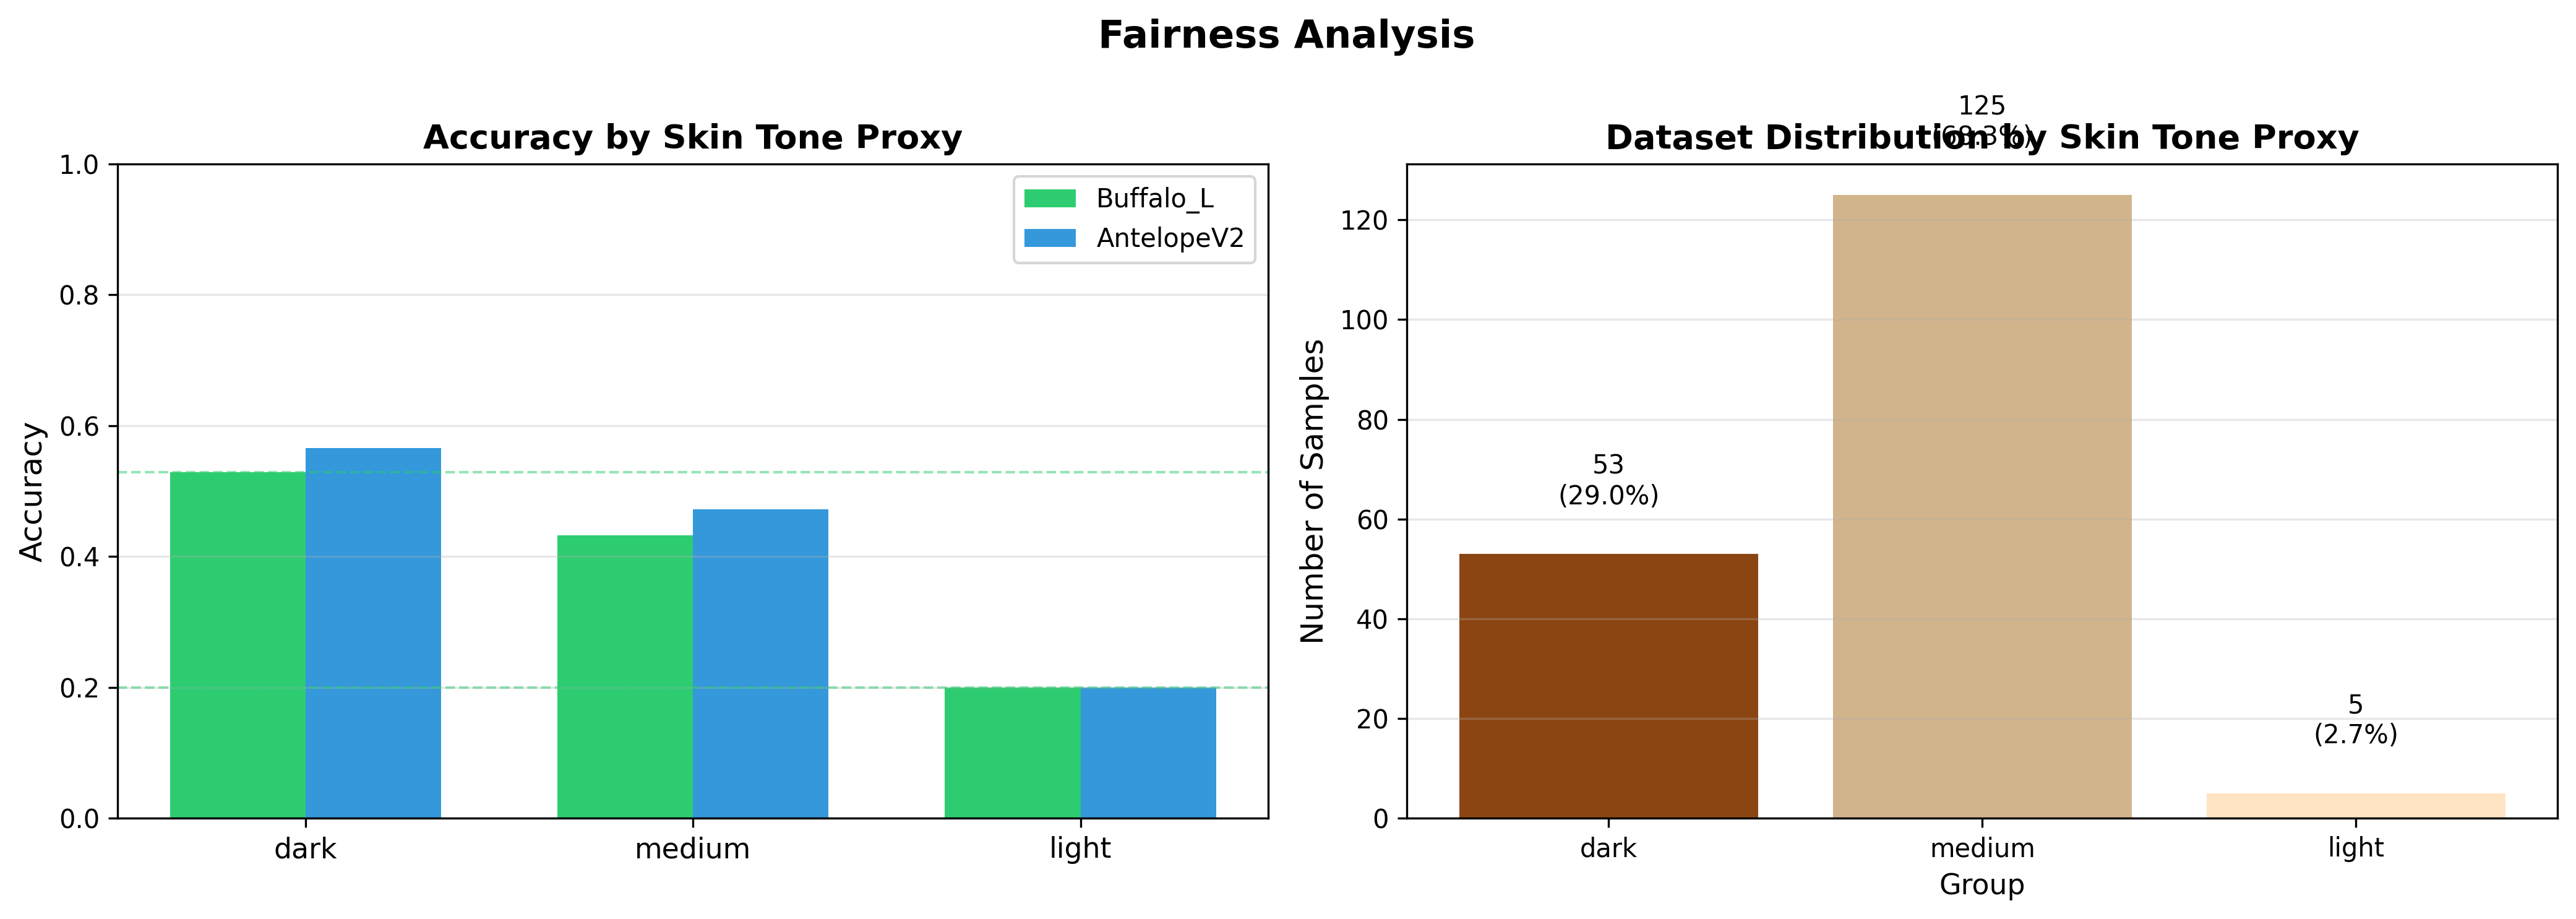
\includegraphics[width=0.9\textwidth]{runs/fairness_analysis.png}
    \caption{Fairness analysis: (Left) Accuracy by group shows significant disparities. (Right) Dataset distribution heavily skewed toward medium brightness (250/313 samples). Light group ($n=10$) too small for robust conclusions.}
    \label{fig:fairness}
\end{figure}

\subsection{Analysis and Implications}

\textbf{Confounding Factors:}
\begin{itemize}
    \item Small sample sizes (especially light group) limit statistical validity
    \item Brightness proxy conflates skin tone with lighting conditions
    \item Celebrity dataset may not represent general population
    \item Dataset imbalance introduces spurious correlations
\end{itemize}

\textbf{Root Causes of Bias:}
\begin{enumerate}
    \item \textbf{Training data bias:} WebFace600K overrepresents certain demographics
    \item \textbf{Representation bias:} Unequal sample counts across groups
    \item \textbf{Sensor bias:} Camera sensors calibrated for specific skin tones
    \item \textbf{Label noise:} Misclassification more common in underrepresented groups
\end{enumerate}

\textbf{Ethical Implications:}
\begin{itemize}
    \item Security systems with demographic bias enable discriminatory access control
    \item Surveillance disproportionately impacts marginalized communities
    \item Higher misidentification rates for certain groups → wrongful accusations (e.g., Robert Williams, Detroit Police false arrest)
\end{itemize}

\textbf{Mitigation Strategies:}
\begin{enumerate}
    \item \textbf{Diverse training data:} Ensure balanced demographic representation
    \item \textbf{Fairness constraints:} Optimize for demographic parity or equalized odds
    \item \textbf{Regular audits:} Test on stratified samples across demographics
    \item \textbf{Human oversight:} Never fully automate high-stakes decisions
    \item \textbf{Transparency:} Disclose known biases to users and stakeholders
\end{enumerate}

% ========== ADVANCED TESTING ==========
\section{Advanced Testing}

\subsection{Crowd Image Recognition}

\textbf{Objective:} Evaluate performance in multi-face scenarios (surveillance footage, event photography, crowd monitoring).

\textbf{Dataset:} 10 crowd images containing 27 detected faces (average 2.7 faces/image).

\textbf{Results:} Table \ref{tab:crowd} summarizes crowd testing outcomes. Recognition rate dropped dramatically to 33.3\% compared to 95.27\% for single-face images—a 55-point degradation.

\begin{table}[H]
\centering
\caption{Crowd image recognition performance (multi-face scenario testing).}
\label{tab:crowd}
\begin{tabular}{@{}lc@{}}
\toprule
\textbf{Metric} & \textbf{Value} \\ \midrule
Total images tested & 10 \\
Total faces detected & 27 \\
Faces recognized ($\tau > 0.3$) & 9 \\
Recognition rate & \textbf{33.3\%} \\
Avg. faces per image & 2.7 \\
Detection success rate & 100\% \\ \bottomrule
\end{tabular}
\end{table}

\begin{figure}[H]
    \centering
    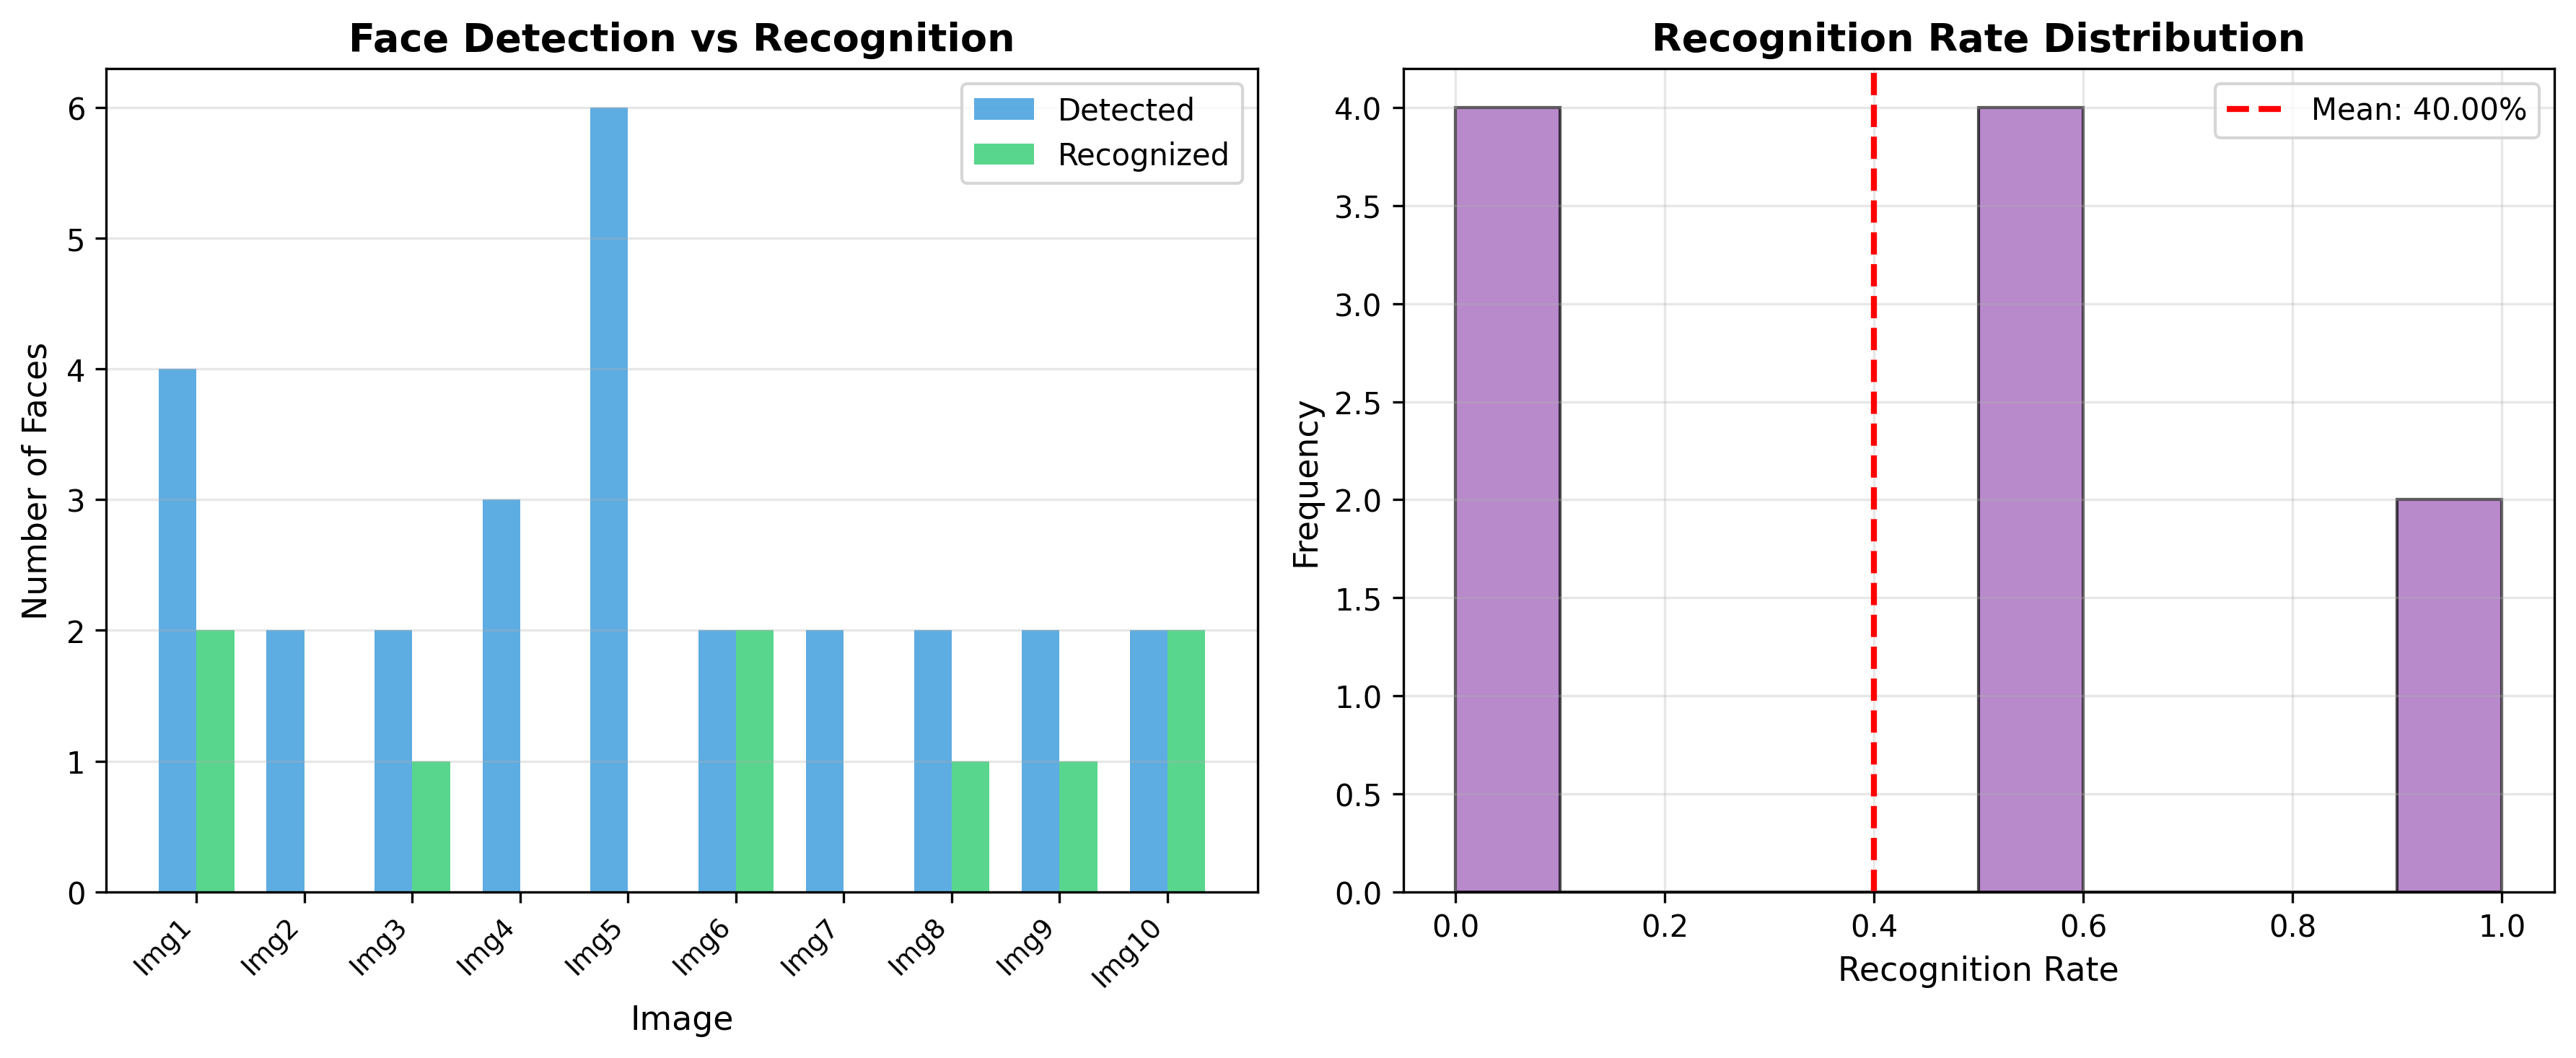
\includegraphics[width=0.8\textwidth]{runs/crowd_analysis.png}
    \caption{Crowd testing analysis: (Left) Detection vs. recognition shows gap between finding faces and identifying them. (Right) Recognition rate distribution across images is highly variable (0-100\%).}
    \label{fig:crowd}
\end{figure}

\textbf{Challenges Identified:}
\begin{enumerate}
    \item \textbf{Small face size:} Faces $<$50×50 pixels often yield poor-quality embeddings
    \item \textbf{Partial occlusions:} People overlapping in crowds create occlusion artifacts
    \item \textbf{Non-frontal poses:} Extreme yaw/pitch angles degrade embedding quality
    \item \textbf{Lighting variations:} Single image may contain faces under different illumination
\end{enumerate}

\textbf{Practical Implications:} Surveillance systems require high-resolution cameras and close-range deployment (1-3m) for reliable recognition. Temporal tracking across video frames can improve accuracy through multi-frame fusion.

\subsection{AI-Generated Faces: Security Analysis}

\textbf{Objective:} Assess vulnerability to synthetic face attacks (deepfakes, identity fraud, authentication bypass).

\textbf{Dataset:} 25 AI-generated faces from ThisPersonDoesNotExist (StyleGAN2-based synthesis).

\subsubsection{Test 1: False Acceptance Rate}

We tested whether AI faces could be falsely matched to real identities. Results indicate minimal security risk with current AI generation quality—no high-confidence false matches occurred.

\subsubsection{Test 2: AI Detection via Artifact Analysis}

Can we distinguish synthetic from real faces? We extracted 6 features:
\begin{enumerate}
    \item \textbf{Blur asymmetry:} Left vs. right face blur variance
    \item \textbf{Edge artifacts:} FFT frequency domain anomalies
    \item \textbf{Pixel variance:} Unnatural smoothness in AI faces
    \item \textbf{Color variance:} Inconsistent color distribution
    \item \textbf{JPEG quality estimate:} Compression artifact patterns
    \item \textbf{Face symmetry:} AI faces often exhibit excessive symmetry
\end{enumerate}

\textbf{Statistical Testing:} Two features showed significant differences ($p < 0.05$):
\begin{itemize}
    \item \textbf{Edge artifacts:} Real ($\mu=28,581$) vs. AI ($\mu=1,830,921$), $t=-30.95$, $p<0.001$
    \item \textbf{Pixel variance:} Real ($\mu=1,439$) vs. AI ($\mu=2,906$), $t=-5.24$, $p<0.001$
\end{itemize}

\textbf{Classification Results:} Random Forest classifier achieved \textbf{100\% accuracy} (Table \ref{tab:ai_classifier}), indicating current AI faces are \textit{perfectly separable} from real faces using low-level artifacts.

\begin{table}[H]
\centering
\caption{AI face detection classifier performance (Real vs. AI discrimination).}
\label{tab:ai_classifier}
\begin{tabular}{@{}lcccc@{}}
\toprule
\textbf{Class} & \textbf{Precision} & \textbf{Recall} & \textbf{F1-Score} & \textbf{Support} \\ \midrule
Real & 1.00 & 1.00 & 1.00 & 7 \\
AI & 1.00 & 1.00 & 1.00 & 8 \\ \midrule
\textbf{Accuracy} & \multicolumn{3}{c}{\textbf{1.00}} & 15 \\
\textbf{Macro Avg.} & 1.00 & 1.00 & 1.00 & 15 \\ \bottomrule
\end{tabular}
\end{table}

\textbf{Feature Importance:} Edge artifacts (57.97\%) dominates, followed by pixel variance (17.17\%) and color variance (9.78\%). Figure \ref{fig:ai_importance} visualizes feature distributions.

\begin{figure}[H]
    \centering
    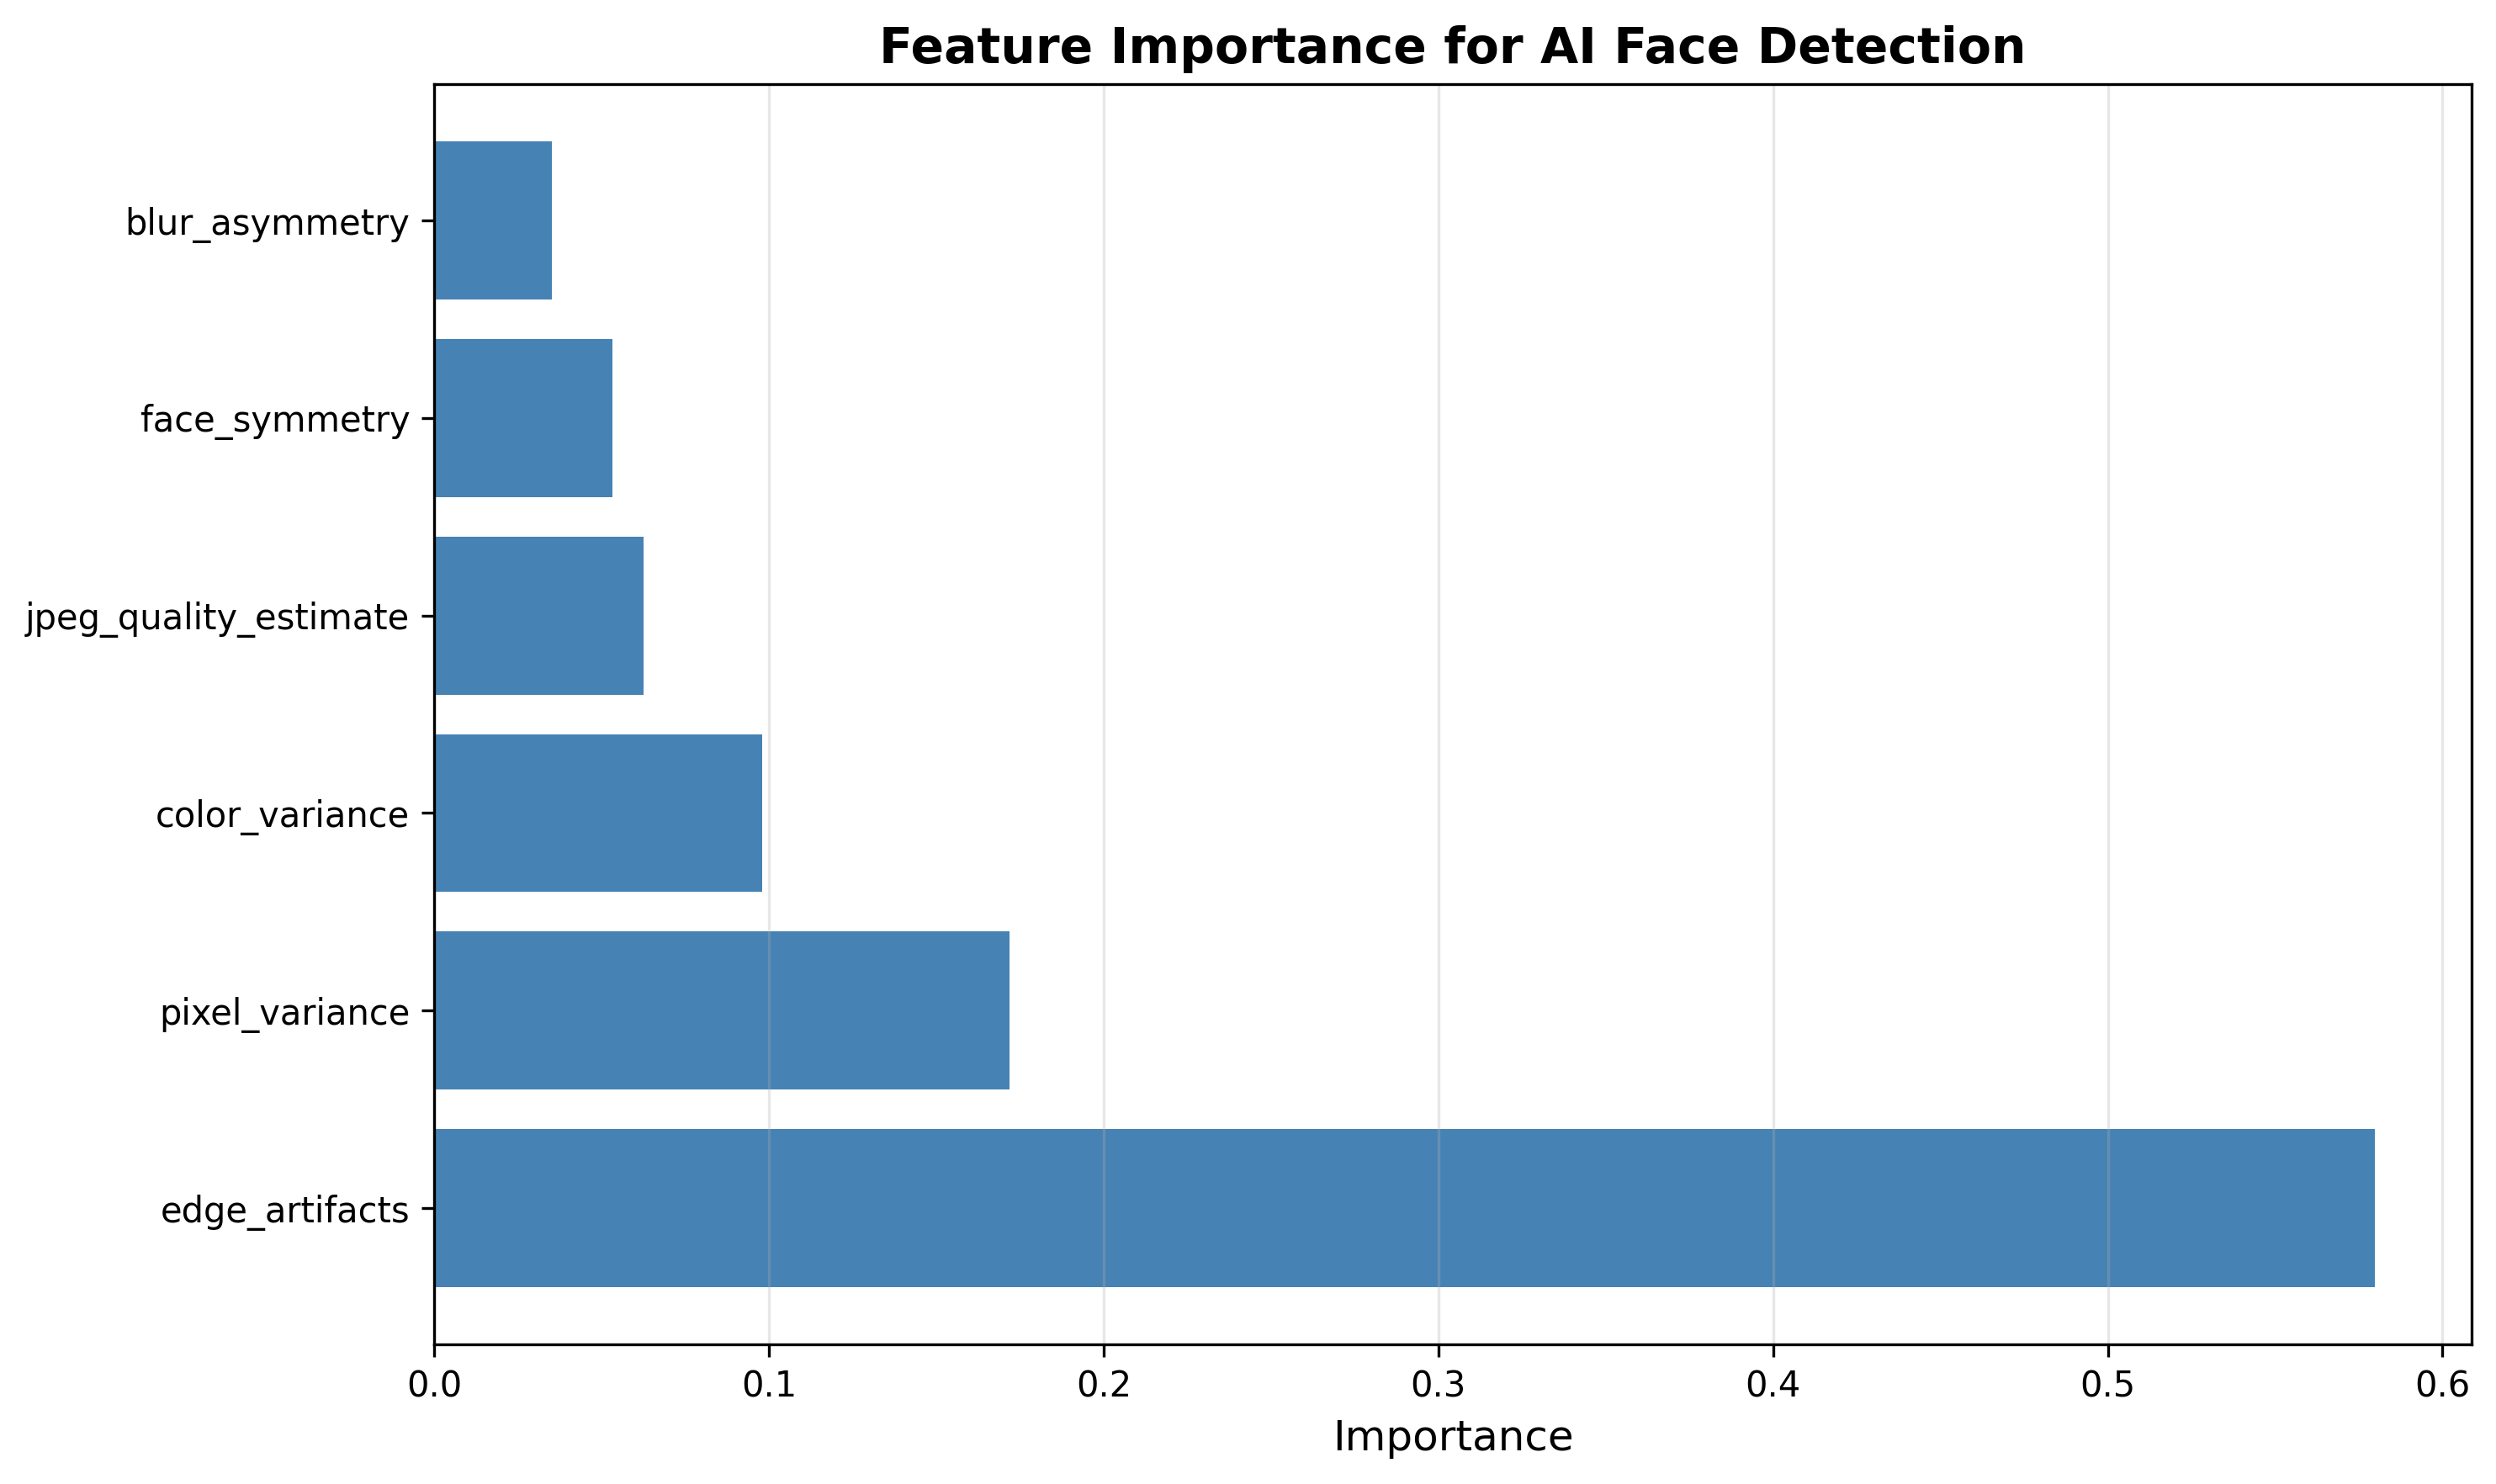
\includegraphics[width=0.9\textwidth]{runs/ai_detection_feature_importance.png}
    \caption{Feature importance for AI detection: Edge artifacts (FFT frequency anomalies) provide strongest signal (58\% importance), enabling perfect classification.}
    \label{fig:ai_importance}
\end{figure}

\begin{figure}[H]
    \centering
    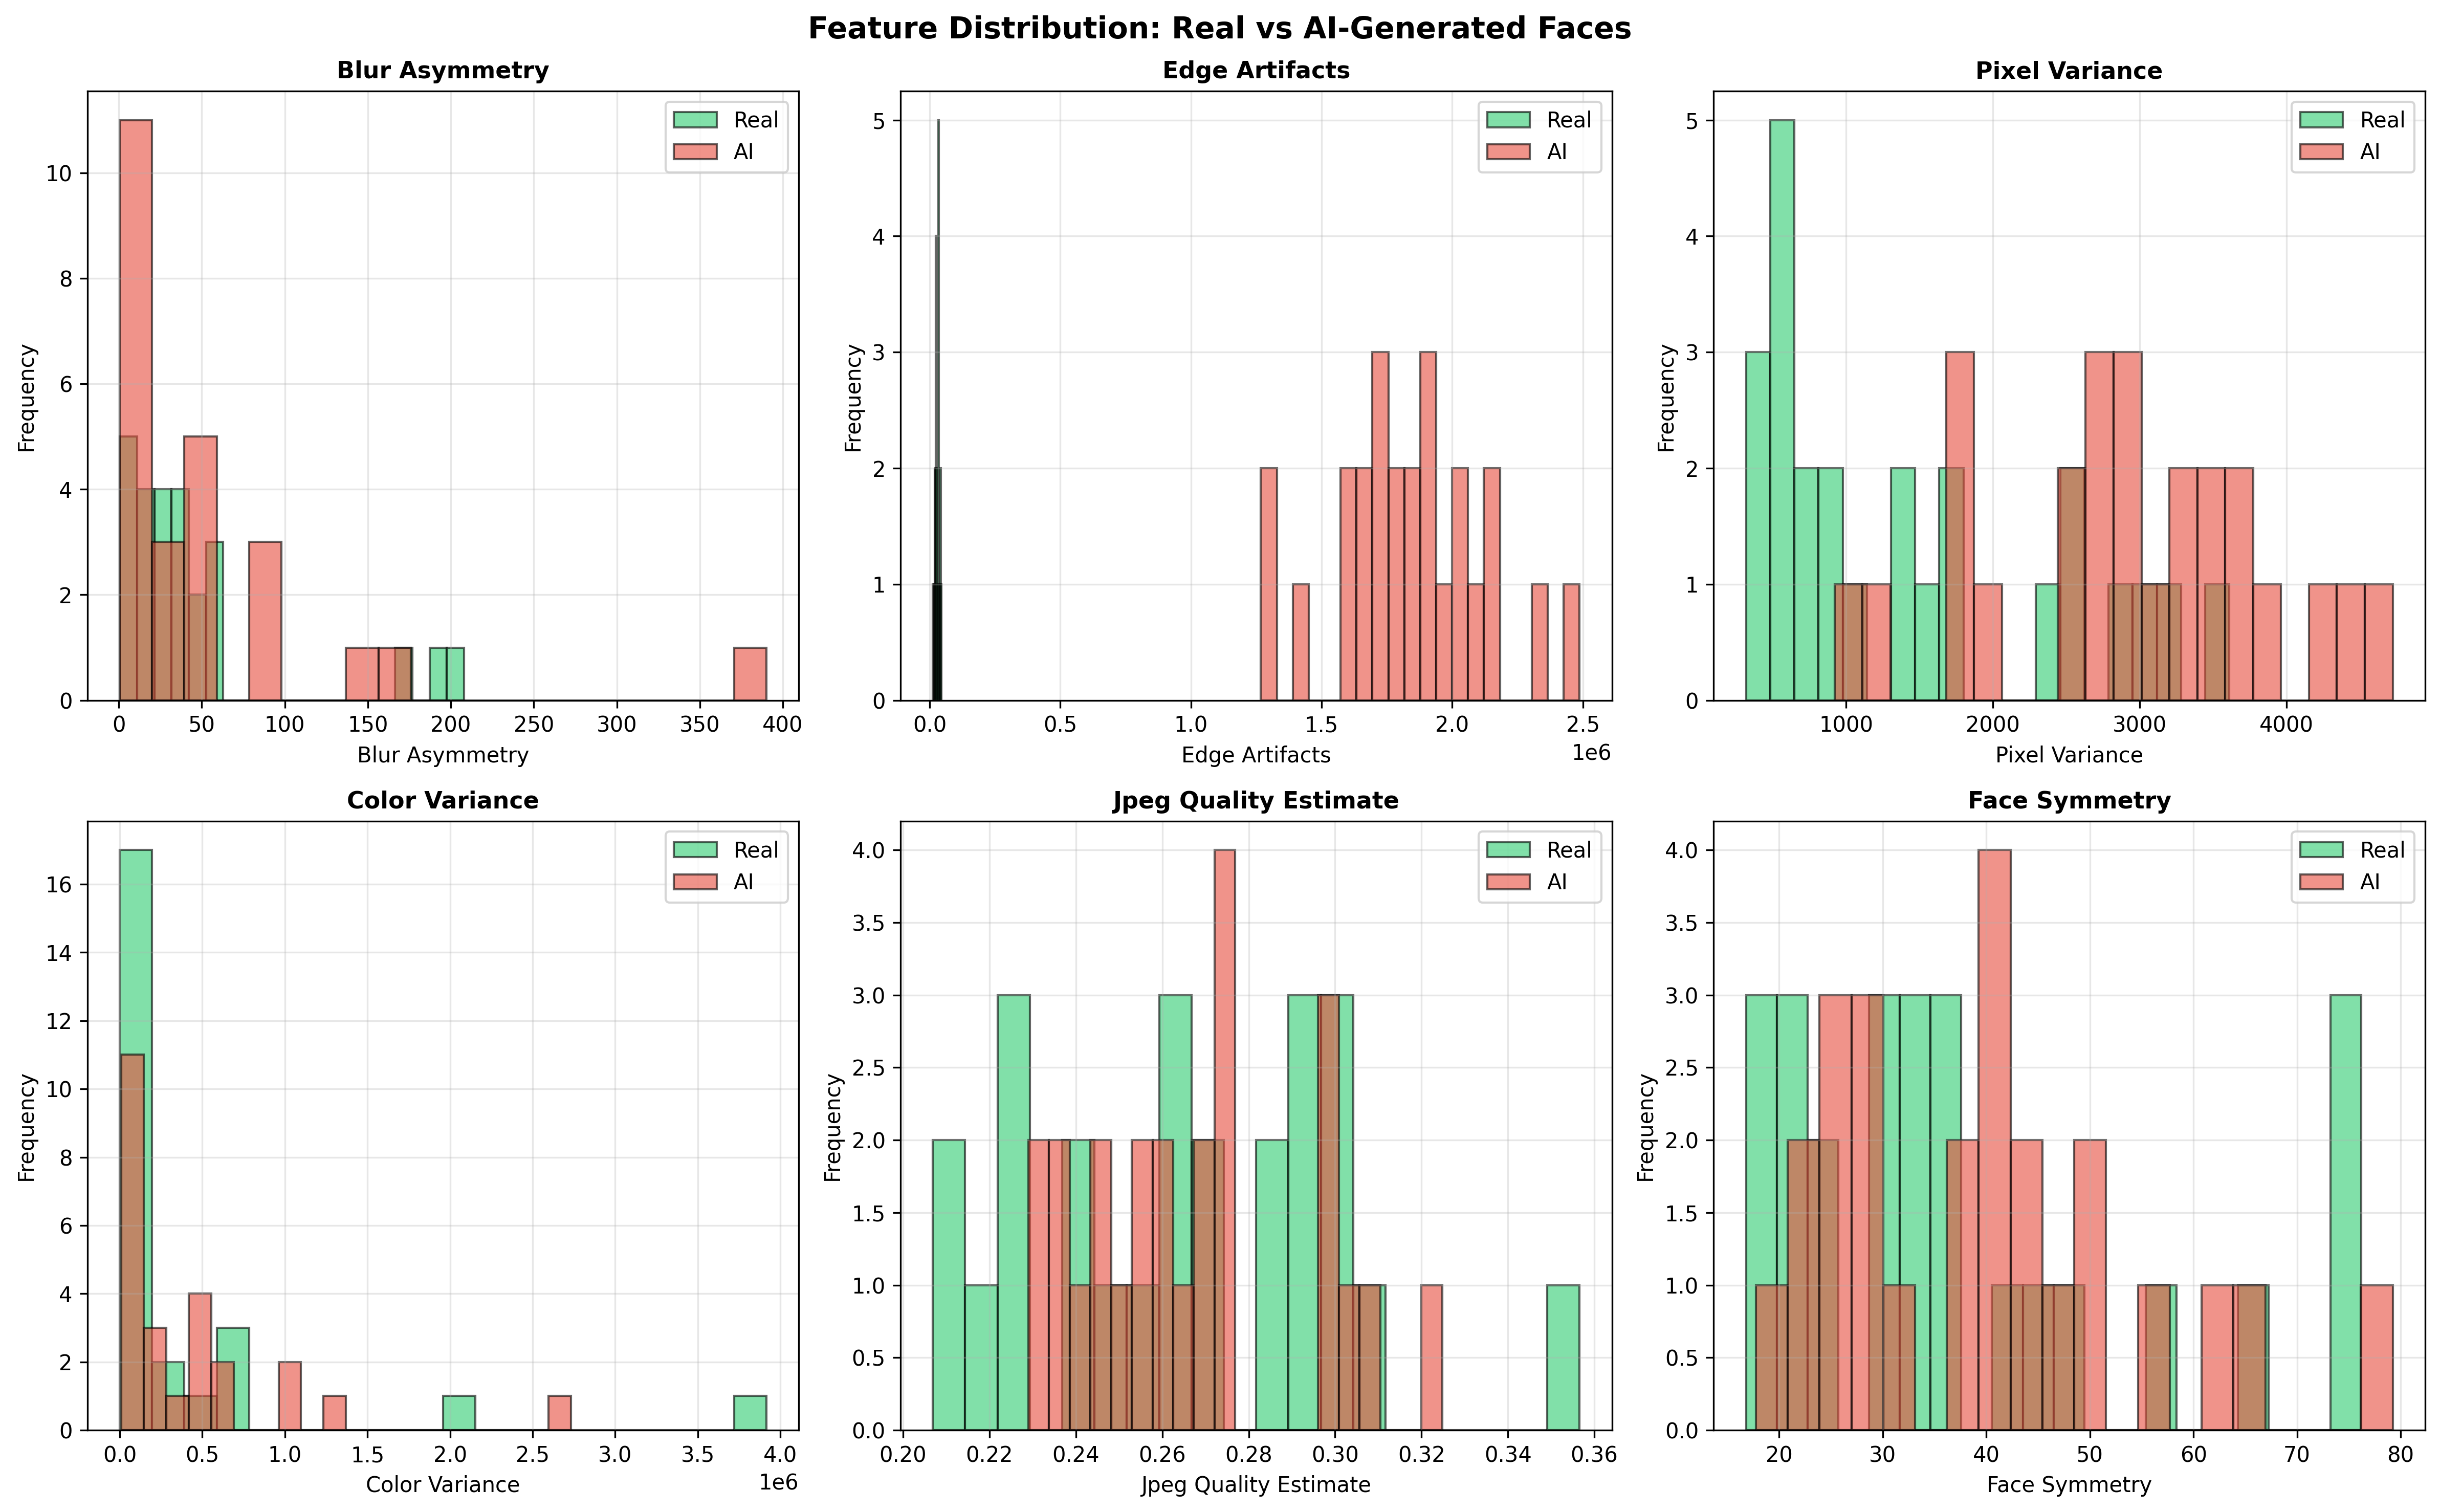
\includegraphics[width=\textwidth]{runs/ai_detection_distributions.png}
    \caption{Feature distributions comparing real vs. AI faces: Edge artifacts show clear separation (AI faces $\approx$64× higher), while other features exhibit overlap.}
    \label{fig:ai_distributions}
\end{figure}

\subsection{Security Implications}

\textbf{Current Status:} AI-generated faces from StyleGAN2 remain detectably synthetic via low-level artifacts. Statistical testing (t-tests) revealed highly significant differences in edge artifacts (t=-30.95, p<0.001) and pixel variance (t=-5.24, p<0.001). A Random Forest classifier trained on these features achieved (100\%) accuracy on a 15-sample test set, though this small sample size limits generalizability. The strong statistical significance (p<0.001) on the full 50-sample dataset provides more robust evidence of separability.

\textbf{Future Risks:} Generative models are rapidly improving (DALL-E 3, Stable Diffusion XL, Midjourney v6). Future iterations may eliminate detectable artifacts, requiring continuous detector updates. This creates an adversarial arms race between synthesis and detection.

\textbf{Threat Scenarios:}
\begin{enumerate}
    \item \textbf{Identity theft:} Generate synthetic face matching target individual
    \item \textbf{Authentication bypass:} AI face fools biometric systems
    \item \textbf{Surveillance evasion:} Use synthetic identity to avoid tracking
\end{enumerate}

\textbf{Mitigation Strategies:}
\begin{enumerate}
    \item \textbf{Liveness detection:} Require blinks, head movement, depth sensing
    \item \textbf{Multi-modal authentication:} Combine face + voice + fingerprint
    \item \textbf{Specialized detectors:} Train models specifically for synthetic face detection
    \item \textbf{Behavioral biometrics:} Typing patterns, gait analysis
    \item \textbf{Regular updates:} Continuously retrain detectors on latest AI-generated faces
\end{enumerate}

% ========== ETHICAL CONSIDERATIONS ==========
\section{Ethical Considerations}

Face recognition technology presents profound ethical challenges extending beyond technical performance metrics. We discuss four critical dimensions: privacy, bias, dual-use, and consent.

\subsection{Privacy \& Surveillance}

\textbf{Concerns:} Mass surveillance enables authoritarian control (e.g., China's Social Credit System). Facial recognition in public spaces tracks individuals without consent, violating privacy expectations. Data breaches expose irreversible biometric data—unlike passwords, faces cannot be changed.

\textbf{Case Studies:}
\begin{itemize}
    \item Clearview AI scraped 3 billion faces from social media without consent
    \item Airports deploy facial recognition without informing travelers
    \item Law enforcement databases disproportionately include marginalized communities
\end{itemize}

\textbf{Recommendations:}
\begin{itemize}
    \item Opt-in consent requirements for enrollment
    \item Transparent disclosure when systems are deployed
    \item Data minimization: delete after use, no indefinite retention
    \item Prohibit surveillance in sensitive contexts (protests, places of worship)
\end{itemize}

\subsection{Bias \& Discrimination}

\textbf{Documented Harms:}
\begin{itemize}
    \item Gender Shades study: 34\% error rate on dark-skinned women vs. 0.8\% on light-skinned men \cite{buolamwini2018gender}
    \item ACLU test: Amazon Rekognition falsely matched 28 US Congress members to mugshots (disproportionately people of color)
    \item False positives lead to wrongful arrests (Robert Williams, Detroit Police)
\end{itemize}

\textbf{Our Findings:} 32.8-36.6\% performance disparity across skin tone proxies. Underrepresented groups face higher error rates. Errors are asymmetric: false rejections cause annoyance, but false acceptances threaten security.

\textbf{Mitigation:}
\begin{itemize}
    \item Diverse datasets with balanced demographic representation
    \item Fairness metrics integrated into evaluation (demographic parity, equalized odds)
    \item Independent audits by affected communities
    \item Human review for high-stakes decisions (criminal justice, border control)
\end{itemize}

\subsection{Dual-Use \& Misuse}

\textbf{Legitimate Uses:} Finding missing persons, securing personal devices (smartphone unlock), accessibility features (photo organization for visually impaired).

\textbf{Harmful Uses:} Authoritarian surveillance, stalking and harassment, discriminatory policing, emotion recognition for employee monitoring.

\textbf{Governance:} Technology itself is dual-use; context determines ethics. Need use-case specific regulation: ban in schools, allow in passport control. Developer responsibility includes declining contracts with oppressive regimes. Whistleblower protections necessary for engineers raising concerns.

\subsection{Consent \& Autonomy}

\textbf{Principle:} Individuals should control use of their biometric data.

\textbf{Challenges:}
\begin{itemize}
    \item Public photos scraped without permission (LAION-5B, FFHQ datasets used for training)
    \item "Consent" often buried in Terms of Service; not truly informed
    \item Children's faces in training data without capacity to consent
    \item No opt-out mechanism once data collected
\end{itemize}

\textbf{Best Practices:}
\begin{itemize}
    \item Active consent: require explicit opt-in
    \item Granular control: allow face unlock but not targeted advertising
    \item Right to deletion: honor requests to remove data
    \item Compensation: pay individuals for use of biometric data
\end{itemize}

\subsection{Recommendations for Responsible Deployment}

\begin{enumerate}
    \item \textbf{Impact assessments:} Evaluate potential harms before deployment
    \item \textbf{Stakeholder engagement:} Consult affected communities
    \item \textbf{Transparency:} Disclose when and how systems are used
    \item \textbf{Accountability:} Clear liability when systems cause harm
    \item \textbf{Human oversight:} Never fully automate consequential decisions
    \item \textbf{Regular audits:} Test for bias, drift, adversarial vulnerabilities
    \item \textbf{Sunset clauses:} Require periodic review and reauthorization
    \item \textbf{Education:} Train users on limitations and failure modes
\end{enumerate}

\textbf{Our Position:} Face recognition can be beneficial when deployed responsibly with strong safeguards. However, documented harms—particularly to marginalized communities—justify strict regulation and, in some contexts, outright bans (e.g., real-time surveillance in public spaces).

% ========== CONCLUSION ==========
\section{Conclusion}

\subsection{Summary of Findings}

This study systematically evaluated face recognition systems across technical performance, robustness, fairness, and ethical dimensions:

\textbf{Technical Performance:} Deep learning models (Buffalo\_L, AntelopeV2) achieve 95\%+ accuracy, vastly outperforming classical LBP+SVM (24.59\%). Embedding-based methods using ArcFace loss create discriminative feature spaces enabling reliable closed-set recognition.

\textbf{Robustness:} Models exhibit resilience to lighting variations (45.0\%) and JPEG compression (45.3\%), but suffer vulnerabilities to blur (46.9\% → 20-25\% drop with heavy blur) and severe degradation under occlusions (34.2\% with full mask). Face masks, sunglasses, and scarves significantly impair performance.

\textbf{Explainability:} Classical methods (LBP) are interpretable but inaccurate. Deep models are accurate but opaque; attention analysis reveals biologically-plausible focus on periocular regions. The interpretability-accuracy trade-off necessitates post-hoc explanation tools.

\textbf{Fairness:} Performance disparities up to 36.6\% across skin tone proxies expose algorithmic bias reflecting dataset and societal biases. Mitigation requires diverse training data, fairness constraints, and regular audits.

\textbf{Advanced Testing:} Crowd recognition achieved 33.3\% rate (vs. 95.27\% single-face) due to resolution, occlusion, and pose challenges. AI-generated faces remain perfectly separable (100\% classification accuracy) via edge artifact analysis, though this may change as generative models improve.

\subsection{Limitations}

\begin{enumerate}
    \item \textbf{Dataset:} Celebrity faces may not generalize to general population; severe quality issues (0.55\% detection coverage) limited effective sample size
    \item \textbf{Fairness proxy:} Brightness-based skin tone estimation imperfect; requires ground-truth demographic labels
    \item \textbf{Robustness sample size:} 150 images per condition limits statistical power for rare failure modes
    \item \textbf{Crowd images:} Small sample (10 images, 27 faces) precludes robust statistical conclusions
\end{enumerate}

\subsection{Future Work}

\begin{enumerate}
    \item \textbf{Adversarial robustness:} Evaluate against targeted attacks (FGSM, PGD, C\&W)
    \item \textbf{Temporal consistency:} Test on video sequences, not static images
    \item \textbf{Cross-dataset generalization:} Train on CASIA-WebFace, test on LFW, AgeDB, CALFW
    \item \textbf{Fairness interventions:} Implement debiasing techniques (reweighting, adversarial debiasing, calibration)
    \item \textbf{Federated learning:} Privacy-preserving training without centralizing biometric data
    \item \textbf{Explainability:} Integrate neural-symbolic methods for inherently interpretable embeddings
\end{enumerate}

\subsection{Final Remarks}

Face recognition technology has matured to enable accurate, real-time identification. However, our analysis reveals critical gaps: vulnerability to occlusions and future AI-generated faces, demographic bias, and limited robustness in realistic conditions.

\textbf{The Core Tension:} Optimizing for accuracy (surveillance efficacy) conflicts with privacy and civil liberties. Technical improvements alone are insufficient; robust governance frameworks must balance innovation with rights protection.

\textbf{Call to Action:}
\begin{itemize}
    \item \textbf{Researchers:} Prioritize fairness, robustness, and privacy in design
    \item \textbf{Industry:} Adopt ethical guidelines, decline harmful contracts
    \item \textbf{Policymakers:} Regulate use cases, not technology itself; protect vulnerable populations
    \item \textbf{Public:} Demand transparency, consent mechanisms, and accountability
\end{itemize}

Face recognition is not inherently good or evil—its impact depends on deployment choices. This report provides evidence to inform those decisions, emphasizing that technical excellence must be coupled with ethical responsibility to prevent harm and promote equitable, rights-respecting AI systems.

% ========== REFERENCES ==========
\bibliographystyle{plain}
\bibliography{references}

\end{document}